\documentclass{report}
\usepackage{scrextend}
\usepackage[parfill]{parskip}
\usepackage{hyperref}
\usepackage[official]{eurosym}
\usepackage{minted}
\usepackage{xcolor}
\usepackage{graphicx}
\usepackage{etoolbox}
\usepackage{framed}
\usepackage{tcolorbox}

\newtcolorbox{ucbox}[2][]
{
    top=-9pt,
    bottom=0mm,
    left=0mm,
    right=0mm,
    colframe = gray!35,
    colback  = gray!15,
    coltitle = gray!30!black,
    title = #2,
    fonttitle=\bfseries,
    parbox=false,
    boxsep=9pt,
    #1
}

\graphicspath{ {images/} }

\def\labelitemi{--}

\def\code#1{\texttt{#1}}

\newcommand{\ucitem}{%
  \par\hangindent3em\hangafter0
  \noindent\llap{$-$\enspace}%
  \ignorespaces
}

\begin{document}


    \title{Stock Management Application (SMAPP)}
    \author{Robert Escuain Poole\\Universitat Politècnica de Catalunya\\Director: Lluís Pérez Vidal}
    \date{\today}
    \maketitle

    \tableofcontents

    \chapter{Context}
    The goal of this project is to design and implement a small-scale free and open-source software solution for stock management. This solution should provide an easy to use platform for small businesses or organizations that need to manage stocks.
If one looks for the definition of stock in, for example, the Merriam-Webster dictionary, the first definition that can be found reads “the supply of goods available for sale in a store” \cite{1}. Although this is a good enough definition, for this project it is better to draw upon the next one, which defines a stock as “a supply of something that is available for use”. Therefore, this project aims to provide a solution for any potential user that needs to manage a supply of something. 

\subsection{Glossary}
Following is a comprehensive list of important terms in the context of this project:

\begin{labeling}{Community member}
\item[POS]{Point of sale. A platform or device used to complete and process a sale.}
\item[Stock]{A supply of something that is available for use.}
\item[Stock management]{(excerpt from The Business Dictionary) The administrative role of assessing the inventory of a business and making sure it is sufficient to meet consumer demand \cite{3}.}
\end{labeling}

\subsection{Stakeholders}
Following are the different stakeholders related to the development, implementation and use of the product, with a description of their roles and functions:

\begin{labeling}{Community member}
\item[Product owner]{Acts as the promoter of the product. Sets the requirements of the product and has the last word regarding its features and functionalities.}
\item[Developer]{Member of the official core team of development. (For this particular project, it will be the same person as the product owner)}
\item[Contributor]{Any developer of the community that submits a contribution to the source code that is accepted.}
\item[Community member]{Any member of the community related to the product that collaborates in any way towards the goal of the project (i.e. reporting a bug, suggesting improvements, giving feedback…)}
\item[User]{The final consumer of the product. This actor has management needs over a particular stock and therefore uses and profits from the product.}
\end{labeling}
    
    \chapter{State of the Art}
    Particularly in this area, there is a really vast amount of software solutions already available, both proprietary and open-source, with paid and free versions, that allow more or less features accordingly. Some of these solutions belong to industry giants long consolidated in their sector, such as SAP and ERP, while others are minor or specialized solutions based on a small scale local market.
While it is good to know about real world use cases and successful solutions, this analysis pretends to focus on the key points these solutions address in order to fulfill each need. In some cases, an actual solution may be mentioned, but due to the huge number of software packages that would be available as an example for each point, it is preferred to overlook them in order to not create noise.

Following are the key points that define a modern stock management solution \cite{5}. These points are now described in a basic and essential manner, but will be explored more in-depth in a technical manner later in the documentation.

\section{Counting and quantifying}
The main function of a stock management solution is to have accurate and comprehensive accounts of the stock, and allow interaction with this data. In short, therefore, a solution has to be able to keep a record of a series of items, which comprise the stock itself, and their current quantities.
On that, the solution should be able to modify these items, in order to add or remove them, or to change their behaviour and identity if needed.
Furthermore, it should allow to modify the quantities. In general terms a decrease in a quantity would mean a sale, while, in order to increase a quantity, an order should be placed. Usually a stock management software solution will add support for both points.
\section{Ordering}
This can also be known as “warehouse flow” in the literature. It is important to have an exhaustive knowledge of the stock, not only regarding quantities, but also regarding categories, types of product, etc, at an abstract or conceptual level. The more comprehensive the management of a stock is, the bigger the impact it has on efficiency and reduction of costs. Therefore features that allow the agile sorting and classification of stock become important.
\section{Reporting}
It is not enough that the software solution is aware of the current state of the stock. The solution must provide an easy and user-friendly way for the people who use it to get a comprehensive and thorough understanding of the state of said stock, in order to control it and react to possible situations and opportunities. Therefore the solution must be able to set and provide significant KPIs.
Regarding this area, alongside the native features that many stock management solutions provide, there are plenty of reporting, analytics and dashboards solutions that can integrate easily with this kind of software. Some of these solutions will be later explored in the project design.
\section{Demand forecasting}
One of the main areas where the efficiency of a stock management system is decided is the one regarding demand forecasting. This concern \cite{7}, addressed perhaps most notably by Toyota in their production chains in Japan during the 1960s and 1970s bases its logic in the principle of stock availability optimization based on the needs of a particular moment.
The paradigm of a warehouse changes from being a platform of massive long-term storage to being a smaller, optimized and temporary housing for a moving good or product. From this rise some principles along the lines of “make only what you can sell”, and “sell only what you can make”. Therefore, software solutions that can provide accurate estimates of both what you can sell and what you can make (and of course, taking into account what you can store) gain a lot of protagonism, and so, along with the recent rise of big data and particularly of data science paradigms many software solutions apply heuristic and trend-aware algorithms in order to provide accurate estimations of the effects from external factors related to the stock, such as increases or decreases in demand, seasonality peaks, etc.
\section{Stock rotation}
Another aspect of stock management is stock rotation. This is particularly important in the food industry, and also with pharmaceuticals and chemicals, and basically any stocks containing perishable goods. These types of stock, having a limited storage life regardless of being sold or not, have to be recurrently renovated. Again, this is reflected in current software solutions in many ways, with features such as periodic order placements. Some of these solutions, like SAP or ERP, include features specific to this concern.
\section{Accessibility}
Perhaps this is not as as obvious a feature as the rest. After all, one could think that the idea is to have the management of the stock near to at the same place as the stock itself. But with the increase in globalization over the last decades and, more recently, the paradigm shift to mobile-first philosophy, easy access to information and tools has become a priority. For instance, particularly in the case of stock management software, ease of integration with handheld devices is a must, alongside multi-platform support of the solution and ease of access from wherever in the world a user might be.
    
    \chapter{Formulation}
    After researching this area, the conclusion is that with the vast amount of existing solutions, it is hard to find a use case that has not been already fully covered. Even with free and open-source solutions, the options, although quite limited in the free version \cite{6,7} or technically speaking \cite{8}, are many.

However, there seems to be a gap in a particular area. All of these solutions are quite rigid and platform specific. They are not easily portable or extendable. There is no solution in the form of an open-source API for basic inventory management, so the goal of this project is to cover this need with a solution that follows this model.

In a similar way, one of the main goals of this project is for it to be free and open-source. The users and clients will not have to pay in order to install and use the software. Support for the software will come from the community that forms around the product, and extra features and extensions of the service and the platform will be built by voluntary contributors.

The solution has to be easy to install and use so the service will be designed as a lightweight standalone solution. That way it can be installed on a single computer with average specifications and served through a local network. The advantage of this is that a client will not need any additional hardware or software dependencies or integrations, and therefore the usage of the service will not imply any additional costs.

Another of the main goals of this service is to be easily extendable so clients with specific needs can implement additional logics and features.

This project will potentially have a positive impact, as it could become a critical platform for the improvement of small businesses and companies that decide to adopt it. While not incurring in extra costs for the users and not representing a noticeable imprint on the environment in any aspect, it can mean a considerable improvement in the efficiency and profits for small users and companies that lack this kind of solution and could not otherwise afford such a system.
    
    \chapter{Scope}
    Based on this apparent need, the overall goal of this project is to design and develop an API based solution, a RESTful service to be more specific, and a proof-of-concept client application that consumes or uses this service in order to provide a solution to an hypothetical user.

The RESTful service will include a running implementation (accessible from internet and running full-time for demo purposes) and its corresponding documentation, which also should be public and also available and accessible. For security purposes, the demo service will only allow read-only calls, but will use an existing environment with realistic data. 

The key traits of the service are the following:

\begin{enumerate}
\item \textbf{Open-source:}
The source code will be hosted on a public repository and (eventually) contributions to the project may be accepted. Any technologies and tools used  on the development of the project have to be strictly open-source.

\item \textbf{Free:}
The product and its use will be free of charges and costs.

\item \textbf{Supported:}
It will be supported by the community it gathers.

\item \textbf{Standalone:}
The solution will be standalone and only require infrastructure from the users, as opposed to a hosted service.

\item \textbf{Multi-platform:}
It will be based on Web technologies in order to provide support to as much platforms as possible.

\item \textbf{Generic:}
As in business-agnostic. The solution should be able to easily integrate with the concept of stock, independently of it being for a shop, warehouse or similar.
\end{enumerate}

According to the characteristics explored on the state of the art, the service will include support for each of these areas in the form of the following features:
\section{Counting and quantifying}
The service will work on and manage a database local to the system, which will store all the data necessary in order to keep track of the inventory. The structure of this data should be easily customizable to be adapted to the needs of different users. The set of features regarding this aspect must also include calls to place orders and account for sales. Support for this includes the need to support providers and customers. This is specified later in this section.
\section{Ordering}
The service must include support for categories and tags in the data structure. Although the structure has to be flexible and adaptable, a minimum set of features and characteristics will be enforced. These features shall be specified in more detail in the technical specification of the service.
\section{Reporting}
The service must allow to build reports on actual data at any given time. Again, the structure and format of these outputs should be as flexible as possible, and therefore the design must be made accordingly.
\section{Demand forecasting}
Support for this feature could reach a very complex level, even more lately with the popularity of machine learning and similar paradigms. For the time being, though, a partial solution will include a feature to set up automatic order placements based on thresholds set by the user.
\section{Stock rotation}
Support for this feature is not intended for the moment. but this area could be covered by a feature to allow time-based periodic order placements. The user of the solution should be able to configure the chronological constraints and customize the orders to place.
\section{Accessibility}
The accessibility issue is addressed by the fact that the solution is a REST service (an API) and therefore can be consumed easily by applications native to a varied and different set of environments, such as mobile apps, desktop apps, other handheld devices, etc.
\section{Support for providers and customers}
The solution has to include a minimal support for the management of provider and customer profiles, upon which orders and sales can be placed.
\section{Possible obstacles}
If the resulting solution is compliant with each and every constraint here described, then it can be considered a useful product. However there are a number of factors that could challenge the success of the project:

\begin{addmargin}[1em]{0em}
\textbf{Support is proportional to community growth:}
Therefore future developments, such as added features or bug fixes, which depend on the community that builds up around the solution, might be little to non-existing, if it doesn’t gain popularity. There is little that can be done in a scenario like this, and this is a common risk with any open source project. The easy way out for this issue if this becomes a problem is to exceptionally allow or provide paid support and third party developments for users that need it and can afford it.

\textbf{Authentication and security:}
This is often one of the greatest challenges in this type of platforms. User trust depends greatly on this aspect, and errors or bad practices in this area might prove very costly. Issues in this aspect might cause users not trusting the platform and therefore the project could end up without having a community. However, given the small reach the platform is expected to have at start, it seems unlikely that it could be targeted by malicious third parties. That said, the design and development of the application will follow as much as possible the good practices and guidelines available in the open source community. Once the platform gains popularity, contributors with expertise on this area can further improve and extend the features needed to provide the necessary security and reliability expected from these kinds of platforms.

\textbf{Input from users and clients:}
While the scope of this project does include an MVP of a product based on the service, as a proof of concept, further solutions and platforms are expected to be developed by the users or third clients. This is not an uncommon problem on open source projects, and not much can be done about it.
\end{addmargin}
    
    \chapter{Work methodology}
    In order to follow and measure the progress of the project, a series of goals will be set along a timeline. These goals will derive on a first basis from the basic features described on the scope of the project. These goals will be iterative and work in a similar way as the sprints in the Scrum methodology:

\begin{itemize}
\item Each goal will be broken down and translated to smaller tasks, until these tasks become atomic enough as to be easily and directly measurable.

\item Each of these tasks will include an estimation of their cost regarding time in order to get an idea of the whole timeline. This should not be enforced in a rigid way, but rather used to provide a way to monitor the progress. 

\item Progress will be measured by the number of the tasks that are considered to be completed. 
\end{itemize}

The project will be successful if all the tasks are completed successfully and therefore all the goals are covered.

As this project will be developed by only one person, at least on the first phase (as described on the scope of the project) there is no need for collaborative work tools.

Regarding planning and success tracking, Trello will be used, although the possibility of using JIRA could be explored.

\section{Validation}
Since the working methodology for the development of this project will be based on Test Driven Development (TDD), the validation of the tasks can be closely related to the software passing correctly the written tests for every use case. 

Therefore there will be an objective way of measuring the success of each development phase: from each requirement a set of use cases will be derived, and for each of these use cases, several features can be specified. In order to be able to implement these features, a test suite for each one has to be written. The task is successful if all tests pass correctly.

As soon as a feature is completed as to cover a use case and complete a goal, these phases can be transferred from a ‘Doing’ section to the ‘Done’ section in Trello or in JIRA, depending on the tool that ends up being used. The project can be considered finished once all the tasks (and by extension all the goals) are ‘Done’.
    
    \chapter{Project outline}
    The deadline for the delivery of the finished project is set on January 9th 2017. Considering the start of the project to coincide with the start of GEP, September 19th 2016, the total duration will be of 16 weeks. The project will be developed using a SCRUM-like methodology, with Sprints of two weeks. Therefore there will be a total of 8 sprints. There will be two spare weeks from the planned end of the project until the official defense. Those two weeks will act as a buffer in case any unforeseen circumstances force a variation in the schedule.
    
    \chapter{Project phases}
    The project planification can be broken down to four main phases: those of Analysis, Documentation \& Specification, Development \& Testing, and the MVP. Following is a more detailed explanation of each one:

\section{Analysis}
The main part of this work will be completed during the GEP Course. This includes the definition of the goal and scope of the project itself, as well as the time planning, economic and environmental studies and presentation of the project. Non-technical documentation is assumed as one of the outputs of this phase, which will span across the first two sprints.

\section{Documentation \& Specification}
During this phase, the design, specification and resulting documentation will be delivered. The documentation will be of a technical nature and consist of three main parts:

\begin{itemize}
\item Use cases, or Functional documentation, which defines the products from a usage point of view: what the product will be able to do, and what it will allow a user to achieve. The expected output of this part, therefore, is a document that will specify the use cases and functional requirements of the designed solution.

\item Architecture design, which defines the product from a technical point of view. This will include the design patterns that will be applied with the justification of their usage, alongside with a diagram of the architecture for a more clear understanding. The expected output of this part is a technical document that describes the architectural design of the solution.

\item User documentation. A user-oriented set of instructions and descriptions meant to make the use of the designed product possible and easy. The expected output of this part is a comprehensive and highly available document describing the features of the designed product and how to use them.
\end{itemize}

This phase will span across sprints 3 and 4 mainly, except for the user documentation part, which will be produced in a coordinated manner alongside the Development phase.

\section{Development \& Testing}
This phase consists of the actual implementation of the solution. It can be also broken down to three main parts:

\begin{itemize}
\item Testing: Against what could seem more intuitive, this can be considered the first part of this phase, as the development will be oriented according to the TDD paradigm. The first step, therefore, is to have a suitable test environment, platform and strategy upon which to carry out the development.

\item Development: This part consists in actually implementing the designed solution and includes, as a first step, the setting up of a local development environment. Also, as per the reasons exposed during the description of the previous part, it will be closely entwined with the testing, so these two first parts will be carried out in a parallel manner. This means that, because of the TDD paradigm, there will be a workload of testing previous to any coding work. Furthermore, as noted before, during this stage it is highly probable that some of the workload will be dedicated to the user documentation, for several reasons: on the one hand, unexpected changes that may arise, and on the other hand, some documentation tools or frameworks may be used to generate said documentation. Usually these tools are used during development time and have presence in the source code itself.

\item Deployment: Once the designed product is implemented and the business logic is correctly working, the next part will be to design and implement an easy process to deploy and make the solution production-ready as easily as possible. Although also implies testing and development like in the previous steps, it can conceptually be considered an altogether different goal. The output of this part includes two aspects: on the one hand, the deployment infrastructure and process itself, and on the other hand, having the solution working in a production environment.
\end{itemize}

This phase will span across sprints 5 and 6 for the testing and development parts, and will use sprint 7 for the implementation of deployment infrastructure.

\section{Consumer MVP}
This final phase has the only goal of providing a proof-of-concept for the whole solution. Since the goal of the product is to provide an easy-to-use solution to be consumed by custom solutions, the output of this phase will be a quick-and-dirty solution that will use the product deployed during sprint 7 and provide an hypothetical profit. This demo will be built during sprint 8. The expected output of this sprint will be a simple client application.

\section{Gantt diagram}
Following is the Gantt diagram outlining the different project phases (Figure \ref{fig:ganttdiagram}) along with a detailed breakdown (Figure \ref{fig:ganttdetail})

\begin{figure}
	\centering
		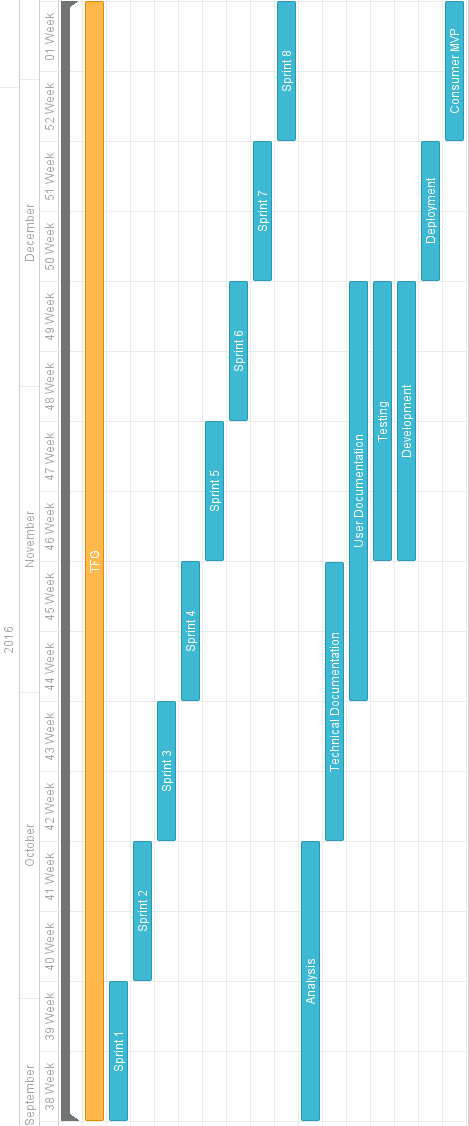
\includegraphics[scale=0.4]{g1.png}
	\caption{Gantt Diagram}
	\label{fig:ganttdiagram}
\end{figure}

\begin{figure}
	\centering
		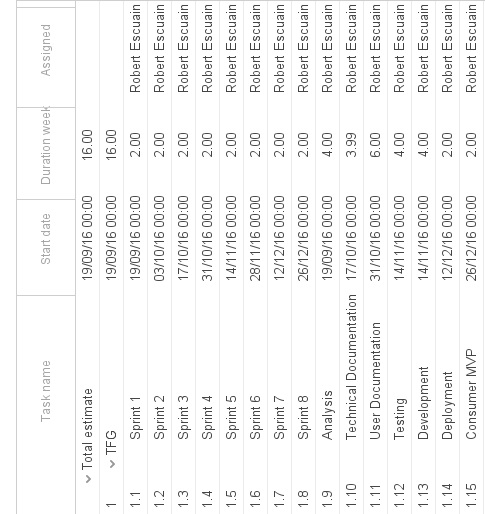
\includegraphics[scale=0.5]{g2.png}
	\caption{Gantt Detail}
	\label{fig:ganttdetail}
\end{figure}
    
    \chapter{Contigency plan}
    Unfortunately there is not much time or room for variations in this planning, because of time constraints. However, at the end of the plan there is a two-week buffer that allows room for corrections in case some of the phases took longer than expected.

It has also to be noted that, although the time estimates for each phase and their parts have been estimated as accurately as possible, some may take more or less. Herein lies the advantage of using an agile methodology, which allows adjusting the schedule and planning more or less at real time, so to say. The initial intention of the plan would be to compensate one time deviation with another one. If one task takes less time than expected, this will allow more margin for other tasks that may take longer, and in reverse.

An additional advantage of using an agile methodology throughout the project is that having more milestones than, for instance, the waterfall paradigm, it is more easy to quickly detect and correct a deviation on the time plan. If deviations like these occur in the middle of the project, measures can be taken on a short notice, and if the deviation is corrected, there is no need to modify the rest of the time plan.

Therefore the idea is to always respect the deadline and compensate during time project, and use the final two-week buffer only as a last resort.
    
    \chapter{Resources}
    Following is a list of the resources which are expected to be used along the completion of the project:

\begin{addmargin}[1em]{0em}
\textbf{Acer Aspire 5735 w. Ubuntu 14.04 LTS}\\
Personal laptop, used mainly for coding on a local development environment and for documentation purposes with an auxiliary character.

\textbf{Custom-build desktop computer w. Ubuntu 14.04 LTS}\\
Personal desktop computer. This will be the main development tool. It will have a local development environment and it will also be used as the usual tool from where to deploy and manage production environments.

\textbf{PHPStorm} (\url{https://www.jetbrains.com/phpstorm})\\
PHP oriented IDE. It will be the main tool for writing and maintaining code.

\textbf{Sublime Text 2} (\url{https://sublimetext.com/2})\\
Text editor. It will mainly be used to manage documentation and configurations, more than code.

\textbf{Vim} (\url{http://www.vim.org})\\
Text editor. It will be used mainly to manage configuration and possibly code on the servers and virtual machines that may be used.

\textbf{Microsoft Word 15}\\
Text processor. Used for documentation purposes.

\textbf{Google Drive} (\url{http://www.google.es/drive/apps.html})\\
Repository used for storing, managing and sharing the documentation.

\textbf{Google Docs} (\url{https://docs.google.com})\\
Used for generating documentation in a shared way.

\textbf{GanttPro} (\url{https://app.ganttpro.com})\\
Online Gantt tool for generating Gantt diagrams.

\textbf{GitHub Account} (\url{https://github.com})\\
Source code repository. It allows to store and manage the source code in a public way, which is a key feature for an open-source project.

\textbf{Trello Account} (\url{https://trello.com})\\
Online tool for task management. It will be used at a personal level to keep track of ongoing tasks.

\textbf{DigitalOcean Droplet} (\url{https://digitalocean.com})\\
Server instance on which the production code will be hosted and run.

\textbf{Google Chrome} (\url{https://www.google.com/chrome})\\
The usual browser used to access the Internet throughout the whole project, for information purposes as well as running and using the client-side infrastructure.

\textbf{Postman} (\url{https://www.getpostman.com})\\
A REST client used for testing the use of REST APIs.
\end{addmargin}

    
    \chapter{Project budget}
    The first step for the elaboration of a budget is to clearly identify the associated costs for every task and resource involved in the project. The goal of the budget is to allow to decide if the project is feasible and makes sense from a cost perspective. The study of the costs includes both human and material resources, as well as possible unforeseen events that might affect the project.

\section{Human resources}
Following are listed the different roles that are involved in the project during the development phase, with their associated cost:
\hfill\break
\begin{center}
    \begin{tabular}{ | l | r |}
    	\hline
 		\textbf{Role} & \textbf{Estimated cost (/hour)} \\ \hline
 		Product owner & 20.00\euro{} \\ \hline
 		Core developer & 16.00\euro{} \\ \hline
    \end{tabular}
\end{center}
\hfill\break
The rest of the roles, as described on the scope and contextualization of the project, have a volunteer involvement on the project, if any, and their involvement is also considered to be after the development phase, and therefore they do not represent any additional cost for the project.

\section{Material resources}
Following are listed the material resources used during the development phase of the project. These include hardware, software and licenses.
\hfill\break
\begin{center}
    \begin{tabular}{ | l | r |}
    	\hline
 		\textbf{Resource} & \textbf{Estimated cost} \\ \hline
 		Acer Aspire 5735 & 499.90\euro{} \\ \hline
 		Custom desktop PC & 1100.00\euro{} \\ \hline
 		PHPStorm & 159.00\euro{}/year \\ \hline
 		Sublime Text 2 & Free \\ \hline
 		Vim & Free \\ \hline
 		Microsoft Word 15 & 149.00\euro{} \\ \hline
 		Google Drive & Free \\ \hline
 		Google Docs & Free \\ \hline
 		GanttPro & Free \\ \hline
 		GitHub Account & Free \\ \hline
 		Trello Account & Free \\ \hline
 		DigitalOcean Droplet & 5.40\euro{}/month \\ \hline
 		Google Chrome & Free \\ \hline
 		Postman & Free \\ \hline
    \end{tabular}
\end{center}
\section{Indirect resources}
Some costs indirectly related to the project must also be taken into account. These costs usually include the connection to the Internet, power, phone calls, transportation, etc. In the case of this project, these resources can be ignored, as they are shared for other purposes and therefore their associated cost becomes negligible.

\section{Other costs}
Usually a budget would also include a margin to cover unexpected conflicts and situations. In this project this would only make sense regarding the human resources (i.e. the analysis or development takes more time than expected), as the material resources are shared with other projects and tasks, and none of them are directly and exclusively related to this project. However, given that the human resources correspond to a student and a tightly defined schedule, any delays and conflicts will have to be covered within the specified dates. The budget can therefore be considered to be rigid regarding the hours.

The budget of this project doesn’t take into account the costs generated by the usage of this project from clients or users once the development phase is finalised.
    
    \chapter{Cost estimation}
    Following the identification of the resources and their costs, a budget estimation can be elaborated taking into account the usage of every resource. The free resources and the resources with no associated cost will be ignored, as the budget only needs to take into account the economical aspect.

In the case of this project, as explained in the scope and contextualization section, the Product owner and the Core developer will be the same person, with some of the functions of each role being tightly coupled with the ones from the other role. Therefore a rough estimation of the different participation has been done.

The total cost in hours for this person is of 420 hours, and it includes the tasks for both roles. Slight variations might occur, but based on the evolution of the project, the estimation can be considered precise enough.
\hfill\break
\begin{center}
    \begin{tabular}{ | l | l | l | r |}
    	\hline
 		\textbf{Resource} & \textbf{Cost} & \textbf{Unit} & \textbf{Total} \\ \hline
 		Product owner & 20.00\euro{}/hour & 120 hours & 2400.00\euro{} \\ \hline
 		Core developer & 16.00\euro{}/hour & 300 hours & 4800.00\euro{} \\ \hline
 		Acer Aspire 5735 & 499.90\euro{} & 3\% * & 14.97\euro{} \\ \hline
 		Custom dektop PC & 1100.00\euro{} & 12.5\% ** & 137.50\euro{} \\ \hline
 		PHPStorm & 159.00\euro{}/year & 20\% *** & 38.10\euro{} \\ \hline
 		Microsoft Word & 149.00\euro{} & 20\% *** & 29.80\euro{} \\ \hline
 		DigitalOcean Droplet & 5.40\euro{}/month & 33\% **** & 1.78\euro{} \\ \hline
 		\textbf{Resource} &  &  & \textbf{7422.15\euro{}} \\ \hline
    \end{tabular}
\end{center}
\hfill\break
{\tiny \textbf{*} Computer used during 8 years. Used during 6 months because of the project, and half of its use is directly related to the project. This yields a rough 3\% usage.}

{\tiny \textbf{**} Computer used during 2 years. Used during 6 months because of the project, and half of its use is directly related to the project. This yields a rough 12.5\% usage.}

{\tiny \textbf{***} Software used for other projects. The 20\% usage is an estimated approximation that takes into account other projects that share the cost of the program, and cannot be disclosed in this budget.}

{\tiny \textbf{****} The service is shared with other ongoing projects. The 33\% usage is an estimated approximation that takes into account other ongoing projects that share the cost of the platform, and cannot be disclosed in this budget.}
    
    \chapter{Cost management}
    Regarding the management of the cost, a strategy must be in place in order to control and oversee the correct evolution of these throughout the project development.

However, in the specific case of this particular project this will not be necessary in some cases. All of the material resources have already been purchased or paid for, and no variations are expected during the project development. If any unforeseen circumstance would however cause further costs in this aspect, it should be taken into account at the end of the project, when the real final costs and the estimated ones are compared.

In this sense, therefore, the hours spent working on the development have to be tracked, both for the Product owner and Core developer roles. This data will also be compared, once the project is finalised, with the estimated amount. Additionally, a precise tracking of the time spent throughout the project can give useful insight and allow corrections of the budget and schedule, in order to adapt and avoid deviations.
    
    \chapter{Sustainability study}
    The sustainability aspect of this project is presented from the following perspectives:

\section{Economic}
\label{sec:131}
The economic study of this project is covered by the budget and cost analysis in the previous sections of this document, which include the total cost and its breakdowns during the whole analysis and development phase. After this phase, the costs associated to the evolution, if any, of the project, can be considered negligible, as all the modifications and support on the product will be in the form of community contributions, which are volunteer. This project will not generate profit or revenue in a direct manner, so it’s not meant to be a competitive product. However, with the advantages of being free and expected to be really easy to use and adapt, it is expected that the product will gather community and a user base.

Regarding the cost levels, it would probably be quite difficult to develop a similar platform with a lower economic cost, as only one person will be in charge of the task. However, the downside of this is that the project will take much longer than if it had a proper development team like a company or a startup could provide. That said, a lot of previous knowledge and experience will go to making the development phase more efficient, as the core developer has gained plenty proficiency in the technologies and tools used throughout the project. After that, further improvements are expected to be contributed by proficient and experienced people from the open-source community.

Given the very low cost and the potential positive impact, the Economic perspective can be valuated with an 8. 

\section{Social}
\label{sec:132}
The goal of this project is to provide an improvement in the tools and platforms used by small companies and stores that cannot afford, or don’t need, or lack the expertise to use more complex and expensive available platforms.

Therefore, if the product is successful, it will be a significant benefit for users that until now have not been able to correctly and precisely track and manage their stocks and products. This will mean, for them, a potential improvement on efficiency and cost management that can result in an increase on revenue. The only disadvantage this product can represent is for other similar platforms (paid, or free but limited) that could see a decrease on their users, if these decide to migrate and start using this new platform.

The small negative consequences for big companies compared to the potentially big impact for smaller users justifies a high score in this perspective, and the valuation for this perspective is an 8.

\section{Environmental}
\label{sec:133}
This project doesn’t have any significant environmental effects, either positive or negative. During the development phase, all of its material resources will be shared with ongoing projects or tasks and so it will not cause an increase in any kind of spending. After that, being the product a very lightweight solution, it is not expected that it will generate any significant consumption of additional hardware, power or any other resource that could affect the environment in a negative way. The solution is expected to work properly on a simple desktop PC based server, and most, if not all, small companies and other users will already be using one. The low impact the project has in this aspect could mean a high valuation for this section. However, even though the project’s influence will not worsen the imprint on the environment, it is not likely that it will improve it significantly. The valuation will therefore be slightly positive, with a 6.

\section{Conclusion}
The conclusion of this study is, that given the particular features of this project, no negative effects or outcomes can be foreseen for the environment, while it could mean a big social and economic improvement for its users, small companies and business owners, with small negative effects on other big and powerful platforms that provide similar services.
\hfill\break
\begin{center}
    \begin{tabular}{ | c | c | c | c | c |}
    	\hline
 		\textbf{Sustainability} & Economic & Social & Environmental & \textbf{Total} \\ \hline
 		Justification & \hyperref[sec:131]{13.1} & \hyperref[sec:132]{13.2} & \hyperref[sec:133]{13.3} & - \\ \hline
 		\textbf{Valuation} & 8 & 8 & 6 & \textbf{22} \\ \hline
    \end{tabular}
\end{center}
    
    \chapter{Architecture of the solution}
    This section presents an explanation on the design of the solution from a technical point of view and the reasons behind it. Its main points are the description of its architecture, followed by an explanation of the framework and the technologies which the implementation is based on, the reasons for it, and the pros and cons of the solution, as well as a more detailed insight on several aspects of the project development and workflow, such as testing, data persistence, deployment and the overall infrastructure.

\section{Why an API?}
Using an API as the core of the solution allows a decoupling that is key to the idea of the whole project. The API will provide access to the business logic in modular ways, giving the potential clients plenty of possibilities to develop or use different features according to their needs.

With libraries like ReactJS, Angular and other similar frameworks it makes sense to provide a backend platform fully decoupled from any frontend. The backend provides the business logic while the frontend decides and defines how the interaction with the user works. Taking this into account, the API is designed with the intention to provide low level decoupled interactions the complete the business logic but don’t condition the interaction with any of them.

In order to further explain this idea, there is a very direct example in the platform that can be used to depict a probable situation. There are two endpoints on the API that are used for increasing or decreasing the stock of a product. At the conceptual level, these endpoints are closely related to buying from a provider (and thus increasing the stock) and selling products to a customer (and thus decreasing it). While it could make sense to have this logic directly coupled to endpoints related to buying or selling orders, having these logics separated, although meaning some extra work in other fronts, makes it easier for different clients with different needs to use these endpoints through their own custom buying and selling logics.

\section{Architecture}
Following is a high-level diagram of the overall architecture for the solution with a general explanation of each of its parts.

\includegraphics[width=\textwidth]{oa.png}

For this particular instance, the app (the API backend) is hosted and run in a dedicated server. The database is also hosted in the same server. This server is managed through and administrator interface. Throughout the development of the project the management has been done through SSH from the administrator computer to the hosting server. From this server the API is exposed, and consumed from two different fronts. 

On on side clients in the main server’s LAN can directly access the API. This would mimic having a server in, for example a warehouse that has also POS’s (points of sale), which would be the computers or devices that access through the same LAN or WAN.

On the other side the API is optionally exposed on the internet so it can be accessed from other devices and client applications. An example scenario for this would be to build a read-only mobile application to view reports and business data from the application.

Note that this design is for the demo implementation. The system is built so it can adapt to different architectures. For example, as it is seen in the diagram, the application and the database are stored in the same server. In other instances the database could be hosted in a dedicated server.

\section{Technologies}
The backbone of the project, the API that implements the business logic of the solution, is implemented in PHP 5.5.9. The reason for using this language among others are that it is very agile and straightforward. Although many would argue in favour of other technologies for projects of this type, the previous experience with this language from the people involved and the requirements of the project, such as speed and simplicity of development, make it a good choice.

\section{Laravel}
Laravel is an open source PHP framework created in 2011 by Taylor Otwell as a more advanced and friendly alternative to Codeigniter and other frameworks from the moment. Although in its initial version it did not provide support for controllers, currently it’s a fully MVC (model-view-controller) oriented framework. Its key features start by being friendly, intuitive and clean, making it pretty straightforward to implement basic and simple applications using only features and capabilities provided out-of-the-box by the framework.

That said, Laravel was not the original decision. Instead the intention was to use its lighter sibling, Lumen, a lightweight version of Laravel that includes the very basics. Although using the light version would be a great opportunity for this project, it lacked a key feature that proved very important. At the moment, Lumen did not support routing on subdomains. This was key requisite in the design application, so the decision to trade lightness for this feature, which is supported on the full Laravel framework was direct.

The key points that established the decision to use this framework for this project are, to begin with, the previous knowledge and experience from the people initially involved, which reduces the learning curve and the time to get a working MVP up and running.

Another decisive feature is the ease to jumpstart, install and deploy the application. Having the right knowledge and experience, taking a simple application from zero to a production environment can take a simple matter of hours, while deploying the basic installation of Laravel is a matter of minutes.

From the API development point of view, the routing features provided by Laravel, described more in detail in the following section, are a big plus.

Also Laravel provides a very straightforward and solid authentication system out-of-the-box. This is again described in more detail in a following section.

As with most of the frameworks, Laravel also provides the order and advantages of a defined file structure, as well as a set of helpers that turn common, often tedious tasks into something easy.

Finally, Laravel also comes with a friendly and intuitive templating engine. However this is not something exploited on this project so no further detail besides mention is needed.

\section{Routing}
One of the most powerful features provided by Laravel is its routing engine. Explained in a simple way, routing consists on assigning the different routes an application has (the addresses used) to their different pages, actions, controllers and so on. These routes are defined in the app/http/routes.php file. For an example, following is the most basic example of a route in Laravel, borrowed directly from the \href{https://laravel.com/docs/5.3/routing}{official Laravel documentation} \cite{9}:

\begin{minted}[frame=lines,framesep=2mm,baselinestretch=1.2,bgcolor=lightgray,fontsize=\footnotesize,linenos]{php}
Route::get('foo', function () {
    return 'Hello World';
});
\end{minted}

So if the base URL for the application were to be www.smappapp.com, this route would cause that going to www.smappapp.com/foo would render ‘Hello World’ in the browser. The simplest route, as in the example provided, is therefore a route and a closure (or callback) function. This callback function can be either defined directly in the routes file or referenced from there.

To reference a particular function you can reference directly a whole controller and the function. This is the case for most of the routes of the application of this project, as seen here, with the main definition for the routes used in the Products features:

\begin{minted}[frame=lines,framesep=2mm,baselinestretch=1.2,bgcolor=lightgray,fontsize=\footnotesize,linenos]{php}
// Products
Route::get('products', 'ProductsController@index');
Route::get('products/{id}', 'ProductsController@find');
Route::post('products', 'ProductsController@store');
Route::delete('products/{id}', 'ProductsController@delete');
\end{minted}

(Note this code was extracted at the time of the documentation for the purpose of an example, and could be outdated)

All the routes on the example reference the ProductsController controller, which contains the business logic related to products and answers to all the actions related to them. As it can be deduced, when reading the code for the controller, the methods index, find, store and delete can be found.

As can also be seen with the example, different HTTP method calls are defined on the routes. Laravel automatically manages the differentiation of these calls, so while the route:

\begin{minted}[frame=lines,framesep=2mm,baselinestretch=1.2,bgcolor=lightgray,fontsize=\footnotesize,linenos]{php}
Route::get('products', ...);
\end{minted}

and:

\begin{minted}[frame=lines,framesep=2mm,baselinestretch=1.2,bgcolor=lightgray,fontsize=\footnotesize,linenos]{php}
Route::post('products', ...);
\end{minted}

will essentially look the same, they are routed to different methods and therefore have different behaviours, as they trigger different methods.

\subsection{Grouping}
Laravel’s routing engine also supports grouping routes, which essentially allows to group routes according to a certain criteria. A very explicit use case for this feature in the application is for adding the API prefix to the routes:

\begin{minted}[frame=lines,framesep=2mm,baselinestretch=1.2,bgcolor=lightgray,fontsize=\footnotesize,linenos]{php}
Route::group(['prefix' => 'api/v1', ...], function() {
	//...
}
\end{minted}

This prefix automatically causes all the routes to add \code{'api/v1'} on the beginning of the route. So while defining the following route:

\begin{minted}[frame=lines,framesep=2mm,baselinestretch=1.2,bgcolor=lightgray,fontsize=\footnotesize,linenos]{php}
Route::get('products', ...);
\end{minted}

will define the action or page for \code{\textless some\_url\textgreater/products}, if we add the route to the grouping, the definition will become the one for \code{\textless some\_url\textgreater/api/v1/products}.

This is very useful for managing APIs, particularly their versions, as there could be different groupings, each one with a different prefix defined for every different version, and with routes that point to the pertinent controllers.

\subsection{Middleware}
The next useful feature of Laravel’s routing is the middleware definition. Middlewares are additional layers that provide logic to the routes. Arguably the most used and popular one is the Auth middleware, that provides authentication logic for the applications. Laravel allows the implementation and injection of custom middlewares but also provides some by default, the Auth one becoming native to Laravel from version 5.1 onwards, due to its popularity and widespread use.

The middleware used for the application is auth:api, an authentication layer for API-oriented application. In order to use the middleware it must be added to the routes. In the application it has been done in the grouping for the API calls:

\begin{minted}[frame=lines,framesep=2mm,baselinestretch=1.2,bgcolor=lightgray,fontsize=\footnotesize,linenos]{php}
Route::group([..., 'middleware' => ['auth:api']], function()
	...
}
\end{minted}

There are several pros and cons to this system. The pros are the ease of use and the code simplicity. The cons are simply that the authentication process is transparent to the developer. This means that if the generic method is enough, there is no problem, but introducing variations or additional features and logic can be a problem.

\subsection{Additional features}
Some very useful additional features related to routing in Laravel are the bootstrapped routes, such as Route::auth(); that will automatically, and in a transparent way, generate all the routes needed for an authentication platform, including login, registering capabilities, password recovery, and so on.

And finally, an indirect perk of this system is that the code itself provides a very clear roadmap of the application that is built. This can be seen either by reading the code itself or, for example, running the following command:

\begin{minted}[frame=lines,framesep=2mm,baselinestretch=1.2,bgcolor=lightgray,fontsize=\footnotesize,linenos]{bash}
php artisan route:list
\end{minted}

The output of this command is a table with the current routes that are in place, as seen in the following example:

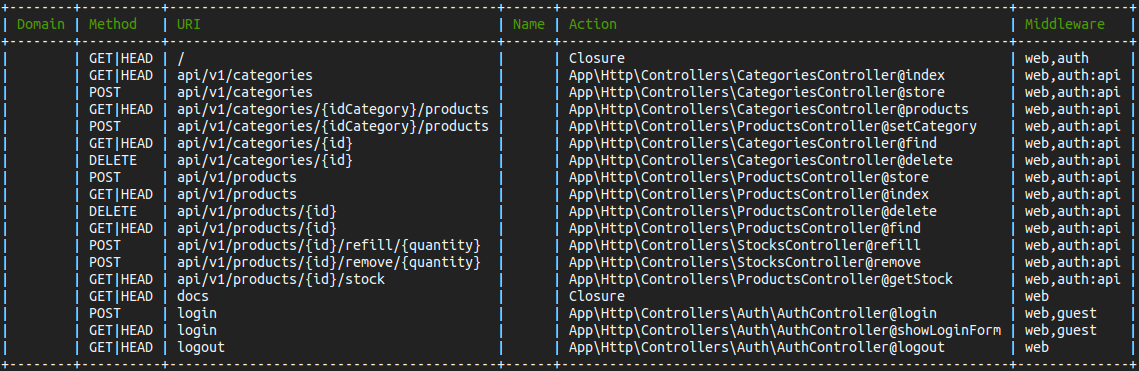
\includegraphics[width=\textwidth]{to.png}

\section{Database}
The database technology of choice for this project is SQLite. There are various reasons for this choice, the most important being the lightness and the simplicity of installation and use. Once the technology is installed, there is no further action required from the user to get it up and running. Although there are several technologies that are often said to be more powerful or reliable for production environments, like PostgreSQL or MySQL, these technologies are slightly more complicated to setup and maintain. Usually SQLite is disregarded for production environments because of its lightness, as if it was a sign of unreliability or the lack of ability to scale. After doing some research, however, there are no reasons to think that SQLite will not perform properly for an architecture and an infrastructure as the one explained in this project.

Taking all this into account, the conclusion is that SQLite offers enough advantages as to be a straightforward decision.

The main advantage of this technology is that the database is basically a single file. That makes it completely standalone and easy to maintain. Backups of the database can consist in merely copying the file to a secure or redundant location. However, if further interaction is required with the database, there are database managers specific to SQLite that can fill this purpose with capabilities like data dumps, data corrections, raw querying, database management and so on.

The native creation, access and management of the database occurs in a transparent way during the installation of the application, and can be done with the default parameters that are already configured in \code{config/database.php} and the \code{.env} file shipped with the standard solution.

The configuration needed for setting up the SQLite database is the following:

\begin{minted}[frame=lines,framesep=2mm,baselinestretch=1.2,bgcolor=lightgray,fontsize=\footnotesize,linenos]{php}
'connections' => [

   'sqlite' => [
       'driver' => 'sqlite',
       'database' => env('DB_DATABASE', database_path('database.sqlite')),
       'prefix' => '',
   ],

],
\end{minted}

This configuration reads the \code{DB\_DATABASE} parameter from the \code{.env} file to set the filename for the database. If the parameter is not found on a \code{.env} file, the default will be \code{database.sqlite} in the \code{/database} folder of the project.

This configuration comes by default with Laravel alongside several other native configurations for different database technologies, specifically MySQL and PgSQL. In order to define SQLite as the technology to be used, it has to be declared as the default with the following line of code, found on the \code{config/database.php} file.

\begin{minted}[frame=lines,framesep=2mm,baselinestretch=1.2,bgcolor=lightgray,fontsize=\footnotesize,linenos]{php}
'default' => env('DB_CONNECTION', 'sqlite'),
\end{minted}

Again, the configuration looks for the \code{DB\_CONNECTION} parameter in the \code{.env} file, and if not found, in the case of this project it defaults to \code{‘sqlite’}.

To change the technologie, the proper tools have to be installed and after that, having the proper configuration in place, the default can be switched to the new technology. The rest is transparent to the user.

Access to the database throughout the application is done through the Eloquent ORM. This ORM comes natively with Laravel and is a simple and straightforward ActiveRecord implementation.

Through Eloquent, every table in the database has a related model through which the application can interact. As an example, for the table \code{products}, there is the \code{Product} model.

Interaction from the application is as simple as follows, in some examples borrowed directly from the code:

\begin{minted}[frame=lines,framesep=2mm,baselinestretch=1.2,bgcolor=lightgray,fontsize=\footnotesize,linenos]{php}
$products = Product::all();
\end{minted}

This line of codes retrieves all the products from the database.

\begin{minted}[frame=lines,framesep=2mm,baselinestretch=1.2,bgcolor=lightgray,fontsize=\footnotesize,linenos]{php}
$product = Product::find($id);
\end{minted}

Here a single, specific product is retrieved, the one identified uniquely by the \code{\$id}.

\begin{minted}[frame=lines,framesep=2mm,baselinestretch=1.2,bgcolor=lightgray,fontsize=\footnotesize,linenos]{php}
$product = new Product();
$product->name = ‘Sample’;
$product->save();
\end{minted}

Here a new product is created, it has a name assigned, and after that is saved and persisted in the database.

\subsection{Migrations}
In order to create the database and its tables Laravel uses what are called migrations. Think of migrations as a version control for database schemas. Tables are created with a schema builder, which allows to define a table and its fields and parameters via source code.

Using that source code, migrations allow to build, create, modify, update, rollback and delete  database schemas in an orderly and coordinated way.

Migrations can be easily created with a command like the following:

\begin{minted}[frame=lines,framesep=2mm,baselinestretch=1.2,bgcolor=lightgray,fontsize=\footnotesize,linenos]{php}
php artisan make:migration create_stocks_table
\end{minted}

This will create a migration outline that will allow adding fields to a specified table, where a developer can define the columns the table needs, as follows:

\begin{minted}[frame=lines,framesep=2mm,baselinestretch=1.2,bgcolor=lightgray,fontsize=\footnotesize,linenos]{php}
public function up()
{
   Schema::create('stocks', function (Blueprint $table) {
       $table->increments('id');
       $table->integer('product_id')->unsigned();
       $table->foreign('product_id')->references('id')->on('products');
       $table->double('quantity')->default(0);
       $table->timestamps();
   });
}

public function down()
{
   Schema::drop('stocks');
}
\end{minted}

The \code{up()} function is used to create the table, while \code{down()} is used to remove it. Upon running the \code{php artisan migrate:refresh} command, Laravel will refresh the migration, meaning that it will rollback what there is via the \code{down()} function, and then create or recreate the table using the \code{up()} function.

When creating the table, the schema builder will set up the columns as specified by the developer in the \code{up()} function.

\subsection{Seeding}
The \code{php artisan migrate:refresh} command can be run with the \code{--seed} parameter. This parameter causes the database to be seeded upon creation.

Seeding a database means filling it with predefined data. This data can be predefined in a wide range of ways using seeders, another feature provided natively with Laravel. Using a seeder a developer can create data to insert at row level, but can also make it to insert autogenerated bulk data.

A simple example for a seeder would be the following, which inserts a single row into the categories table, using a randomly generated 10-digit string for the name column and a 100-digit one for the description column:

\begin{minted}[frame=lines,framesep=2mm,baselinestretch=1.2,bgcolor=lightgray,fontsize=\footnotesize,linenos]{php}
public function run()
{
   DB::table('categories')->insert([
       'name' => str_random(10),
       'description' => str_random(100),
   ]);
}
\end{minted}

The \code{run()} function is invoked by the \code{DatabaseSeeder} class, the native seeder provided by Laravel.

\section{Authentication}
The authentication of the API is done by using an API token.  This token is unique for each user inside an installation of the application. By default, when the application is installed, and as part of the process, a default administrator user is created via a seeder to act as the default client of the API. Credentials for this user are documented in the installation documentation, alongside instruction on how to log in and retrieve its unique token.

To grant access to the API to clients it is enough to share this token. Client users and applications have to set this token in a header for every call done to the API. If the token belongs to a user in that particular system, the call can be  run. This means that there is no way to access other instances of the API even when possessing some valid token.

The authentication itself is managed by Laravel’s \code{auth:api} middleware, native in version 5.2. Any passwords are stored encrypted in the database with one-way encryption using the bcrypt library.

The basic implementation of the API does not manage different access roles or clearance levels at the moment, but in the future a feature like this is a must-have. The authentication logic should be able to allow read and write privileges separately, instead of full or no access, for security purposes.

\section{Testing}
Testing has a key role throughout the development of this project, as the work methodology approach has been the one of TDD, or Test Driven Development. 

The basic principle of this paradigm is to build the tests before writing the production code. Although it’s a debate open to plenty of discussion for many different communities, this presents the developer team with many advantages, being the main one the need to have a clear idea of what is being built before building it. Another consequence of this methodology is that the output, if done right, is clean and orderly code. This approach also causes, in a sort of subconscious way, to structure the architecture of the application in a sensible modular way. 

All in all, TDD is a set of principles and guidelines that, well applied, provide many advantages towards clean code.

In order to build a comprehensive suite of tests on which to base the correctness of the code and its features, a testing framework has been integrated into the application.  The framework of choice is Codeception.

Codeception is a testing framework that provides elegant and efficient testing capabilities for PHP source code. Its election as the framework of choice are due to its direct and native integration with Laravel. Installing and starting to using it is a very straightforward process.

After installing it via Composer, some configuration has to be done over the default one, adapting the test logic to the scenario. In the case of this project, the application is being tested by a suite of acceptance tests that work directly on the API behaviour.

For this the only particular tweaks needed were the addition of a helper to manage the database (the tests occur in a temporal environment which uses the real development database) and browser capabilities, which are provided by PhpBrowser

\subsection{Configuration}
Besides the default configuration, therefore, it is enough to add and configure the Db helper as follows:

\begin{minted}[frame=lines,framesep=2mm,baselinestretch=1.2,bgcolor=lightgray,fontsize=\footnotesize,linenos]{php}
modules:
   config:
       Db:
           dsn: 'sqlite:./database/database.sqlite'
           user: ''
           password: ''
           dump: tests/_data/dump.sql
           populate: false
           cleanup: true
\end{minted}

In this configuration, the dsn field points to the database that is being used. The other fields that are important are populate, which specifies if the database needs to be prepared with data prior to the testing, which in this case is false, and cleanup, which indicates if the database has to be rollbacked, or cleaned, once the tests have finished. To avoid inconsistencies with the development and manual testing, the database is always cleared before and after the tests, so the tests are agnostic to any other factors that otherwise could condition them, such as leftover data from seedings or manual tests, or even normal use of the API during development stages.

Once Codeception is configured to work on the project, a specific test suite is created with the following command:

\begin{minted}[frame=lines,framesep=2mm,baselinestretch=1.2,bgcolor=lightgray,fontsize=\footnotesize,linenos]{php}
php codecept generate:suite api
\end{minted}

This will generate a suite which will contain all the tests specific to the API (all of them, in the case of this project).

This suite needs specific configuration of its own, which is the following, and can be found directly on the \code{/tests} folder:

\begin{minted}[frame=lines,framesep=2mm,baselinestretch=1.2,bgcolor=lightgray,fontsize=\footnotesize,linenos]{php}
class_name: ApiTester
modules:
   enabled:
       - \Helper\Api
       - Db
       - REST:
           url: http://localhost:8000/api/v1
           depends: PhpBrowser
           part: Json
\end{minted}

This configuration enables the API, Db and REST helpers, which are features that allow the easy testing of API based features. Enabling Db here allows the use of the Db helper configured earlier at the Codeception level.

\subsection{Tests}
Once Codeception is installed and configured, and a test suite is defined, the actual tests can be written. Codeception provides an intuitive syntax that makes code easy to write and easy to understand afterwards. As an example, this is the code that tests the correct creation of a product:

\begin{minted}[frame=lines,framesep=2mm,baselinestretch=1.2,bgcolor=lightgray,fontsize=\footnotesize,linenos]{php}
public function CreateProductTest(ApiTester $I)
{
	//...

	$I->wantTo('create a product via API');
	$I->haveInDatabase('categories', $sampleCategory);
	$I->sendPOST('/products', $sampleProduct);
	$I->seeResponseCodeIs(\Codeception\Util\HttpCode::OK); // 200
	$I->seeResponseIsJson();
	$I->seeResponseContains('"errors":false');
	$I->seeInDatabase('products', $sampleProduct);
}
\end{minted}

Some code, basically the preparation of the data for the test, that is the \code{\$sample\_} variables and the authentication process have been omitted, for cleanliness and security purposes. However, the full test suite can be found in the source code.

Once the tests are written, they can be run with the following command:

\begin{minted}[frame=lines,framesep=2mm,baselinestretch=1.2,bgcolor=lightgray,fontsize=\footnotesize,linenos]{php}
composer exec codecept run api
\end{minted}

Assuming the production code necessary to pass the test is correct, and the test passes, Codeception will display something similar to this:

\begin{minted}[frame=lines,framesep=2mm,baselinestretch=1.2,bgcolor=lightgray,fontsize=\footnotesize,linenos]{php}
ProductsCest: Create a product via api (0.24s)
\end{minted}

However, if there are errors while executing the tests, Codeception will display a comprehensive explanation of what went wrong, as follows:

\begin{minted}[frame=lines,framesep=2mm,baselinestretch=1.2,bgcolor=lightgray,fontsize=\footnotesize,linenos]{php}
---------
1) ProductsCest: Check the stock of a product via api
 Test  tests/api/ProductsCest.php:GetProductStock
 Step  See response contains json {"errors":false,"product_id":"1","quantity":100}
 Fail  Response JSON does not contain the provided JSON
- array (
  'errors' => false,
  'product_id' => '1',
  'quantity' => 100,
)
+ array (
  'product_id' => 1,
  'quantity' => '100.0',
  'errors' => false,
)
Failed asserting that false is true.

Scenario Steps:

 7. $I->seeResponseContainsJson({"errors":false,"product_id":"1",...})
 6. $I->seeResponseIsJson()
 5. $I->seeResponseCodeIs(200)
 4. $I->sendGET("/products/1/stock",[])
…

FAILURES!
Tests: 18, Assertions: 60, Failures: 1.
\end{minted}

The test result shows that there is a format inconsistency between the response of the API and the expected results, as well as detailing the step in which the inconsistency has been detected (see lines 9 and 13).

The next step in the development, therefore, would be to fix this explicit bug. Once all the tests are passed, one of the options is to create a new test for a production feature. After writing the test, the whole test suite should be run again, and the new test should fail. This means the test is testing something that’s new to the current implementation and therefore adds value. If the new tests doesn’t fail it can mean that either the test is no well written, or that the feature the test checks is already implemented, and therefore the new test is redundant.

The other option is to refactor the current code in order to optimise it or make it more clean. After any modification to the code, the test suite can be run again to make sure nothing in the production implementation has broken as a result of code changes. This results in a very solid and reliable code base.

\section{Deployment}
One of the requirements of the whole solution is for it to be easy to set up and install. The effort required from the user should be minimal, and therefore the process has to be automated as much as possible.

So far the designed solution is supported to be installed in a machine running a late version of Ubuntu. It is designed so only a couple of manual steps are required, which are very simple and are well explained in the \code{readme.md} of the project repository.

The installation process, however, assumes a specific set of requirements are met. These requirements are also listed in the \code{readme.md} and include having Apache 2, PHP (\textgreater= 5.6.4), and Composer to begin with. From here, the environment has also to fullfill Laravel's own requirements, which include:

\begin{itemize}
\item OpenSSL PHP Extension
\item PDO PHP Extension
\item Mbstring PHP Extension
\item Tokenizer PHP Extension
\item XML PHP Extension
\end{itemize}

Although it is not a mandatory requirement for Laravel, the \code{php5-sqlite} library is needed, since the default application uses SQLite for the database.

Once these requirements are met, the project has to be cloned in a suitable folder inside \code{/var/www/}. This will create a file named \code{smapp}, which contains the application. Inside the folder, under the \code{installation} folder, there is an installer, \code{install.sh}, and a VHost configuration file, \code{smapp.conf}. The user has to manually modify \code{smapp.conf} according to the instructions inside, basically setting up the domain under which the application will be called, and optionally setting up a custom name for the application. After this is done, the user simply has to run the installer to complete the installation.

Once the script has finished running, the application will be installed and ready to use.

\subsection{The install.sh script}
Most of the installation process is automated with the following simple script:

\begin{minted}[frame=lines,framesep=2mm,baselinestretch=1.2,bgcolor=lightgray,fontsize=\footnotesize,linenos]{php}
appname="smapp" # MODIFY APPNAME HERE (OPTIONAL)

# DO NOT MODIFY BELOW THIS LINE ########################

mv smapp.conf /etc/apache2/sites-available/$appname.conf

a2ensite $appname.conf

service apache2 reload

mkdir bootstrap/cache

sudo chgrp -R www-data storage bootstrap/cache
sudo chmod -R ug+rwx storage bootstrap/cache

/usr/local/bin/composer.phar install

touch database/database.sqlite

php artisan migrate:install

sudo chgrp -R www-data database
sudo chmod -R ug+rwx database

php artisan migrate:refresh --seed -n --force

mv .env.production .env

php artisan key:generate
\end{minted}

By order, this script does the following tasks:

\begin{itemize}
\item Moves the VHost file to its correct location.
\item Enables the new configuration and reloads Apache 2 for the changes to have effect.
\item Prepares directories and their correct permissions before the application installation.
\item Installs the application itself.
\item Creates and sets up the SQLite database with the correct permissions for the application.
\item Sets up the environment-specific configuration.
\item Generates a key for the application to authenticate to itself.
\end{itemize}

Once these tasks are successfully completed the application is fully deployed and ready to use.

\section{Online resources}
As well as the technical documentation for the API, a key resource is the client documentation that provides definitions and instructions to follow in order to use the API. In the case of this project, this resource is exposed online alongside the API itself, and can be found \href{http://smapp.sorters.io/docs}{here}.

This documentation is a static HTML file generated automatically using the RAML (RESTful API Modeling Language) language and the \code{raml2html} tool. RAML is a language that allows designing and specifying an API in a friendly and intuitive way. It uses YAML as the syntax of the documentation source files. As well as defining the API, it allows to generate the documentation in an automated way, and with the raml2html tool it is easy and straightforward to turn it into a static HTML page.

The basic documentation, the header so to say, for an API will look similar to the following example:

\begin{minted}[frame=lines,framesep=2mm,baselinestretch=1.2,bgcolor=lightgray,fontsize=\footnotesize,linenos]{php}
#%RAML 1.0
title: SMAPP

baseUri: http://smapp.sorters.io/api/{version}
version: v1
mediaType: application/json
protocols:
 - HTTP
\end{minted}

With this fragment of code, the title of the API Documentation is set, alongside the base Url used for consuming the API, its version, the media type of its responses, and the protocols it supports.

Once the basics are documented, each endpoint of the API can be described in detail. For example, the \code{/products/\{id\}} endpoint documentation is along the lines of the next example:

\begin{minted}[frame=lines,framesep=2mm,baselinestretch=1.2,bgcolor=lightgray,fontsize=\footnotesize,linenos]{php}
/products/{id}:
 uriParameters:
   id:
     description: The unique identifier for the Product.
     type: integer
     example: 27

 get:
   description: List details of a Product.
   responses:
     200:
       description: The details of a Product.
       body:
         type: Product
     401:
       description: Unauthorized
     404:
       description: Not found

 delete:
   description: Deletes the Product.
   responses:
     200:
       description: The deletion was successful.
     401:
       description: Unauthorized
\end{minted}

This examples describes two different methods for this endpoint, the GET and the DELETE, which correspond to HTTP calls. It states that for both (therefore this is a shared endpoint) an ID parameter is needed.

After that, separately for each method call, it describes every possible response, with its HTTP response code, and the body and details of the response.

Note in the GET description that the body is described with a type, which is a Product. This is because RAML allows to declare entities described separately, similar to classes or objects. The definition for the type Product would look like this:

\begin{minted}[frame=lines,framesep=2mm,baselinestretch=1.2,bgcolor=lightgray,fontsize=\footnotesize,linenos]{php}
Product:
 description: A Product
 properties:
   id:
     description: A unique identifier for the Product.
     type: integer
     example: 27
   name:
     description: A unique name for the Product.
     type: string
     example: Keyboard
   description:
     description: A description for the Product.
     type: string
     example: Wireless standard QWERTY keyboard
   category_id:
     description: The identifier of the Category to which the Product belongs, if any.
     type: integer
     example: 3
     required: false
   created_at:
     description: The date when the Product was first created.
     type: datetime
     example: 2016-12-02T15:01:12Z
   updated_at:
     description: The date when the Product was last modified.
     type: datetime
     example: 2016-12-06T12:33:52Z
\end{minted}

This information (note how placeholder data is provided as examples for each attribute) will later be used in the HTML page to be able to simulate requests and responses in an interactive way, making the documentation richer with actual realistic examples, which makes the API easier to understand and grasp.

The following command can be run in order to do a build of the documentation and obtain the HTML source code for the static documentation page:

\begin{minted}[frame=lines,framesep=2mm,baselinestretch=1.2,bgcolor=lightgray,fontsize=\footnotesize,linenos]{php}
raml2html docs/smapp.raml > docs/smapp.html
\end{minted}

The resulting page is a self-contained HTML file with its own styles and the source code needed to showcase the API described.

\section{Infrastructure}
For the hosting of the solution and the documentation, DigitalOcean has been the technology of choice. The key factors for this decision have been the previous successful experience with the platform  and its ease of use, as well as the transparency of its costs. Apart from all this, it is easy to select a plan from the range of the offer the service provides that adapts to the specific needs of the application.

The application is hosted on a droplet (a virtual instance) in the AMS3 datacenter in Amsterdam. The dedicated instance has 512MB of RAM, a 20GB SSD hard drive, a single core processor and 1TB available for data transfer. This is the minimal instance, but more than enough for the application to run and respond smoothly with the expected workload.

The droplet is running Ubuntu 14.04.3 x64. The application is served by apache2, which was installed manually. As the instance was empty on startup, Apache, PHP, SQLite and the curl and bcrypt libraries had to be installed manually. However, the application would be able to run on any server with a generic LAMP installed.

The server hosts other projects, so this application was assigned a subdomain. In order to access the API using the subdomain, the VHost configuration had to be particularly modified. The configuration is as follows:

\begin{minted}[frame=lines,framesep=2mm,baselinestretch=1.2,bgcolor=lightgray,fontsize=\footnotesize,linenos]{php}
	ServerName smapp.sorters.io
	DocumentRoot /var/www/smapp/public
	<Directory /var/www/smapp/public>
		Options Indexes FollowSymLinks MultiViews
		AllowOverride All
		Allow from all
	</Directory>
\end{minted}

With this, all the requests against smapp.sorters.io is redirected to Laravel’s \code{/public} folder, and from there processed using the rules of the routing table explained earlier.

The only additional variation to Laravel’s native structure has been to expose the API user documentation with the \code{/docs} endpoint via a static HTML, as explained on the Online Resources section.

The management of the droplet is through SSH from the development computer.

The source code is hosted on GitHub, to easily make it available to the open source community.
    
    \chapter{Feature analysis}
    From the areas described in Chapter 4: Scope of this project, a series of features can be defined, alongside their use cases. Being that the final product of this project is an API, the only actors here involved will be the Client and the System. The Client interacts with the System by doing calls to a series of endpoints that are provided by the API as an interface to the business logic of the solution. Also, for all use cases, the precondition of the Client being authenticated (logged in) in the System is assumed and will not be explicitly listed.

The use cases here described provide an abstraction of the business logic and are agnostic to the actual implementation. Therefore the names used for the endpoints of the API or different features of the system may not coincide with the actual implementation. For the technically accurate documentation of the System please refer to the Technical Documentation of the API, which will be exposed as part of the implementation.

The use of the term describe in the following sections refers to listing the attributes and their values for the elements it refers to. So \textit{describing} a product means listing the attributes of a product alongside the value of each one of them.

\section{Counting and quantifying}
For this feature, two entities arise: the Product and the Stock. The product is an abstraction of the goods that are being managed by the Client in his business, while the Stock is an abstraction for the actual existence of these goods. A product can have many stocks, the most usual case being to have a stock for each batch purchased. This allows a better tracking of the existences of the product, and where it comes from.

To further clarify, in an hypothetical case there is a Client who manages Product A, but doesn’t have any in the warehouse, so has no Stock of this product. He has Product A, but no Stock of Product A. Once he has purchased a number (N) of items of Product A, he will have a Stock of N Product A’s. While still having this stock, the Client purchases another number M of items of Product A. Now he has two stocks of Product A, one with N and another with M items. The total stock of Product A is N+M.

The most essential use cases when managing products are related to knowing what is exactly being managed in the system. There must be a feature that allows listing all the available products, and another one that allows getting all the information about a specific product. Additionally, upon a base of existing products, a user has to be able to create and add new products, and also modify any of the existing ones. Finally, there has to also be support for deleting existing products from the system.

The resulting features for products, in the form of use cases, which are described in detail in the annex, are the following:
\hfill\break
\begin{itemize}
\item \hyperref[UCP001]{UCP001: List Products}
\item \hyperref[UCP002]{UCP002: Describe Product}
\item \hyperref[UCP003]{UCP003: Add Product}
\item \hyperref[UCP004]{UCP004: Modify Product}
\item \hyperref[UCP005]{UCP005: Delete Product}
\end{itemize}
\hfill\break
Regarding stocks, it is also required to be able to list them all, in order to provide hindsight of the bigger picture, if needed. A more critical feature, however, is to be able to view the existing stocks of a specific product. For this purpose, as described earlier, stocks are considered independent quantities of a product. In this particular case this is designed in this way to provide awareness on a practical level. Different stocks will represent, for instance, different batches of a product, usually bought and received at different moments in time.

However, when referring to the stock or current stock of a product, in singular, it will mean to absolute quantity of units of that product available. A specific feature should allow to retrieve this information.

Additionally, stocks should be increasable and decreasable. Stock increases are not a problem, because either the increase has to be done in a specific stock (determined in a manual way, so to say, by its ID) or the increase is represented by the creation of a whole new stock. However, stock decreases represent a problem because there must be a logic that determines from which of the available stocks the quantity should be removed. The native implementation for this will be a FIFO (first in, first out), so a given quantity will be removed starting from the oldest stock available.

The resulting features regarding stocks, in the form of use cases, and detailed also in the annex, are as follow:
\hfill\break
\begin{itemize}
\item \hyperref[UCS001]{UCS001: List all Stocks}
\item \hyperref[UCS002]{UCS002: View Product Stocks}
\item \hyperref[UCS003]{UCS003: Get Product Stock}
\item \hyperref[UCS004]{UCS004: Add to Product Stock}
\item \hyperref[UCS005]{UCS005: Remove from Product Stock}
\end{itemize}
\hfill\break
Indirectly, the features described in this section provide indirect support for purchases and sales via the increase or decrease of the product stock. Although further support for this kind of transactions may be implemented natively in the solution, exposing this step will allow potential contributors to integrate different logics for purchases and sales, in conjunction with the logic that supports providers and customers, described later in its section.

\section{Ordering}
For this feature, two different entities appear: Categories and Tags. 

A product can (but not must) belong to at most one category. As can be deduced by the name, categories help categorize different types of products according to certain characteristics. These categories are customized and managed by the user.

This capability implies first a feature to list all the available categories. A user should be able to add to this categories by creating new ones, and also to modify existing ones. Additionally, a user should be able to remove and delete categories.

A product can be assigned to a category when creating or modifying it. If a product is assigned to a category and that category is changed, the previous relationship ceases to exist, as one product can only belong to a single relationship. 

This implies some features that allow knowing about this relationship. From one side, to know what category a specific product is assigned to, and from the other side of the relationship, which products are assigned to a specific category.

The features for categories, in the form of use cases, are described in more detail in the annex and are as follow:
\hfill\break
\begin{itemize}
\item \hyperref[UCC001]{UCC001: List Categories}
\item \hyperref[UCC002]{UCC002: Describe Category}
\item \hyperref[UCC003]{UCC003: Add Category}
\item \hyperref[UCC004]{UCC004: Modify Category}
\item \hyperref[UCC005]{UCC005: Delete Category}
\item \hyperref[UCC006]{UCC006: List Products of Category}
\item \hyperref[UCC007]{UCC007: Assign Category to Product}
\end{itemize}
\hfill\break
In a similar way to categories, a product can have multiple tags assigned. Tags will represent an abstraction of a particular trait (temporary or not) that can be shared by multiple products across different categories. A specific scenario that showcases the use of tags could be a marketing campaign that affects a certain number of products. In order to easily identify these products, they can be assigned the tag related to the campaign while it lasts.

Tags are not explicitly created. A tag comes to exist when it is assigned to a product. The reason for that is agility on the process. While categories are something more structured that require previous thought and design, the idea for the tags is they are to be used on the spot. Not having to create a tag before assigning it makes the process more agile, but less strict. This means a user has to use this logic with discretion, as it can easily lead to unmaintainable and unscalable inconsistencies, if not managed properly.

A user also needs to be able to untag a product, by removing the tag from it. However, the tag will continue to exist.

As with the categories, features have to enable to see the relationships between products and tags. A feature has to list the tags assigned to a product, and for the other way around, a feature has to list all the products that are tagged with a specific tag.

These requirements imply the following features:
\hfill\break
\begin{itemize}
\item \hyperref[UCT001]{UCT001: Assign Tag to Product}
\item \hyperref[UCT002]{UCT002: Remove tag from Product}
\item \hyperref[UCT003]{UCT003: Get Products by Tag}
\item \hyperref[UCT004]{UCT004: List Product Tags}
\end{itemize}
\hfill\break
Further detail can be found in the annex, where this features are described in the form of use cases.

\section{Reporting}
The requirements for this section state that the service must allow to build reports on the current data at any given time. The features originating as a consequence from this will mostly use features from the other sections, typically the ones that refer to listing, filtering and ordering.

Because of this, the features needed to fulfill these requirements can be completely based on the use cases of the other sections. Therefore this section will list the external features used, with the implication that they are however adapted to meet the purposes of this section, meaning that the response is expected to be in the form of reports.
\hfill\break
\begin{itemize}
\item \hyperref[UCP001]{UCP001: List Products}
\item \hyperref[UCS001]{UCS001: List all Stocks}
\item \hyperref[UCS003]{UCS003: Get Product Stock}
\item \hyperref[UCC001]{UCC001: List Categories}
\item \hyperref[UCC006]{UCC006: List Products of Category}
\item \hyperref[UCT003]{UCT003: Get Products by Tag}
\item \hyperref[UCT004]{UCT004: List Product Tags}
\item \hyperref[UCTR001]{UCTR001: List Triggers}
\item \hyperref[UCPP001]{UCPP001: List Providers}
\item \hyperref[UCCU001]{UCCU001: List Customers}
\item \hyperref[UCPO001]{UCPO001: List Purchase Orders}
\item \hyperref[UCPO008]{UCPO008: List Purchase Lines from Purchase Order}
\item \hyperref[UCPO009]{UCPO009: List Purchase Lines by Product}
\item \hyperref[UCPO010]{UCPO010: List Purchase Lines by Provider}
\item \hyperref[UCSO001]{UCSO001: List Sale Orders}
\item \hyperref[UCSO002]{UCSO002: List Sale Orders by Customer}
\item \hyperref[UCSO009]{UCSO009: List Sale Lines from Sale Order}
\item \hyperref[UCSO010]{UCSO010: List Sale Lines by Product}
\end{itemize}
\hfill\break

\section{Demand forecasting}
Support for this feature could reach a very complex level, even more lately with the popularity of machine learning and similar paradigms. For the time being, though, a partial solution will include a feature to set up automatic order placements based on thresholds set by the user.

Therefore this implies a set of features that implement a CRUD logic on an entity that will represent triggers, with thresholds to be checked each time the stock of a product is modified. Apart from creating, listing, updating and deleting these triggers, a user has to be able to enable and disable them, depending on if the thresholds have to be checked or not the next time the stock is intervened, and the triggers activated.

Configuring a trigger means specifying a threshold, or the minimum stock below which an action has to be triggered. The action will be by default, on the native implementation, to place an order for a certain quantity of a product to a specific provider. All these parameters are part of the configuration of the trigger entity.

The resulting features, which are further detailed in the annex in the form of use cases, are as follow:
\hfill\break
\begin{itemize}
\item \hyperref[UCTR001]{UCTR001: List Triggers}
\item \hyperref[UCTR002]{UCTR002: Describe Trigger}
\item \hyperref[UCTR003]{UCTR003: Add Trigger}
\item \hyperref[UCTR004]{UCTR004: Modify Trigger}
\item \hyperref[UCTR005]{UCTR005: Enable Trigger}
\item \hyperref[UCTR006]{UCTR006: Disable Trigger}
\item \hyperref[UCTR007]{UCTR007: Delete Trigger}
\end{itemize}
\hfill\break
\section{Stock rotation}
Support for this feature is not intended for the moment. but this area could be covered by a feature to allow, for instance, time-based periodic order placements. The user of the solution should be able to configure the chronological constraints and customize the orders to place.

\section{Support for providers and customers}
For the features in this sections, two main entities will be created, those of Provider and Customer.

The Provider entity is the most important of both because order placements are assigned to them. When creating an order to increase the stock of a product, a Provider has to be selected and this Provider will be the one whom the order is submitted to. Therefore a full CRUD feature is needed in order to be able to manage providers. Also, besides listing all the providers registered in the system, a user has to be able to list the specific details of a single provider.

The features for managing providers, therefore, are the following:
\hfill\break
\begin{itemize}
\item \hyperref[UCPP001]{UCPP001: List Providers}
\item \hyperref[UCPP002]{UCPP002: Describe Provider}
\item \hyperref[UCPP003]{UCPP003: Add Provider}
\item \hyperref[UCPP004]{UCPP004: Modify Provider}
\item \hyperref[UCPP005]{UCPP005: Delete Provider}
\end{itemize}
\hfill\break
In a different way, while the Customer entity can be important, it’s not mandatory. It can be used for Customer Relationship Management, or CRM, or in other words to keep track of who the products have been sold to. A full CRUD feature is again needed for this entity.

The resulting features for customers are the following:
\hfill\break
\begin{itemize}
\item \hyperref[UCCU001]{UCCU001: List Customers}
\item \hyperref[UCCU002]{UCCU002: Describe Customer}
\item \hyperref[UCCU003]{UCCU003: Add Customer}
\item \hyperref[UCCU004]{UCCU004: Modify Customer}
\item \hyperref[UCCU005]{UCCU005: Delete Customer}
\end{itemize}
\hfill\break
Both sets of features can be found described in more detail, as use cases, in the annex.

\section{Sales and Purchases}
This section covers the features that allow the system to manage purchases to providers, and sales, either to specific customers or not. For this, several entities will be used. Although this logic could belong in the Counting and Quantifying section, it is documented separately as it depends on features from several other sections. 

On the purchases side, there will be Purchase Orders, which will include Purchase Lines, each Purchase Line representing a product bought to a provider.

A purchase order is created when the user needs to process purchase lines. A purchase line is created by the user in order to increase the stock of a given product. A line is created specifying the product to be purchased and the provider from which it will be purchased. There are two ways to have a purchase line in an order, either directly adding them as parameters when creating the purchase order (on the POST body, in the case of this project) or creating them separately with a specific feature, and then adding them to an existing order with another specific feature. This can be found explained in the user documentation of the API.

By default, a purchase line will have a state of open, which means that it is pending processing. In a similar way, if an order has open lines, its state will also be open. This implies features to manage the state of both lines and orders. Additionally, a user might need to change lines from an order to another, as well as modifying these orders. Finally, a user has to be able to delete both lines and orders. To delete a line or an order, those have to be in a state of closed.

These orders have to be visible, and besides listing all the orders, all the lines, and the lines of a specific order, a user has to be able to list purchase lines for a specific product and for a specific provider.

Once purchase lines are ready to be processed (usually this is when the user receives the goods from the provider) a purchase line can be acknowledged. This results in the stock for that product being increased and the purchase line’s state to be changed to closed.

Following is a summarized list of features that originate in this section. These features are described in the annex in the form of use cases.
\hfill\break
\begin{itemize}
\item \hyperref[UCPO001]{UCPO001: List Purchase Orders}
\item \hyperref[UCPO002]{UCPO002: Describe Purchase Order}
\item \hyperref[UCPO003]{UCPO003: Create Pruchase Order}
\item \hyperref[UCPO004]{UCPO004: Edit Purchase Order}
\item \hyperref[UCPO005]{UCPO005: Close Purchase Order}
\item \hyperref[UCPO006]{UCPO006: Open Purchase Order}
\item \hyperref[UCPO007]{UCPO007: Delete Purchase Order}
\item \hyperref[UCPO008]{UCPO008: List Purchase Lines from Purchase Order}
\item \hyperref[UCPO009]{UCPO009: List Purchase Lines by Product}
\item \hyperref[UCPO010]{UCPO010: List Purchase Lines by Provider}
\item \hyperref[UCPO011]{UCPO011: Describe Purchase Line}
\item \hyperref[UCPO012]{UCPO012: Create Purchase Line}
\item \hyperref[UCPO013]{UCPO013: Edit Purchase Line}
\item \hyperref[UCPO014]{UCPO014: Assign Purchase Line to Purchase Order}
\item \hyperref[UCPO015]{UCPO015: Acknowledge Purchase Line}
\item \hyperref[UCPO016]{UCPO016: Delete Purchase Line}
\end{itemize}
\hfill\break
On the sales side, there will be sales, which include sale lines. A sale can be assigned to a specific customer or not.

A sale is created because an actual sale is happening or has happened. A sale includes one or more sale lines, each one for a specific product. Full sales, not sale lines, are optionally assigned to customers. This is different from purchases with providers, where the lines and no the order refer to the providers, and the reason for this is that usually one wouldn’t make a sale of multiple products to multiple customers, while it is common to make a purchase order of a set of products bought to different providers.

Sales can be created as completed or as pending. The first case would be useful, for example, in scenarios like a supermarket, where the sale is done on the spot, while the second case would be for orders that can take time to deliver. This implies state for the orders, and features to manage this states.

Features for listing all the sale orders, their lines, and the lines according to a criteria, such orders by customer or sale lines by product, are also needed. These orders and lines, in a similar way as to purchases, have to be modifiable and deletable.

Finally, alike the feature that allows to acknowledge received purchase lines, a similar feature is needed to acknowledge sale lines. Once a line is delivered, and therefore the order for that product is fulfilled, this feature will change the state of the order to closed, and will reflect the sale on the stock of that product, decreasing by the quantity of the product sold because of the line.

As a result, the following features are originated:
\hfill\break
\begin{itemize}
\item \hyperref[UCSO001]{UCSO001: List Sale Orders}
\item \hyperref[UCSO002]{UCSO002: List Sale Orders by Customer}
\item \hyperref[UCSO003]{UCSO003: Describe Sale Order}
\item \hyperref[UCSO004]{UCSO004: Create Sale Order}
\item \hyperref[UCSO005]{UCSO005: Edit Sale Order}
\item \hyperref[UCSO006]{UCSO006: Close Sale Order}
\item \hyperref[UCSO007]{UCSO007: Open Sale Order}
\item \hyperref[UCSO008]{UCSO008: Delete Sale Order}
\item \hyperref[UCSO009]{UCSO009: List Sale Lines from Sale Order}
\item \hyperref[UCSO010]{UCSO010: List Sale Lines by Product}
\item \hyperref[UCSO011]{UCSO011: Describe Sale Line}
\item \hyperref[UCSO012]{UCSO012: Create Sale Line}
\item \hyperref[UCSO013]{UCSO013: Edit Sale Line}
\item \hyperref[UCSO014]{UCSO014: Assign Sale Line to Sale Order}
\item \hyperref[UCSO015]{UCSO015: Acknowledge Sale Line}
\item \hyperref[UCSO016]{UCSO016: Delete Sale Line}
\end{itemize}
\hfill\break
Further detail can be found on the annex, where these features are listed in the form of use cases.
    
    \chapter{Domain description}
    This section follows as the next step in the evolution from the conceptual domain explored in the feature analysis section and provides a lower level technical description of the classes and general architecture originated from it. Although this is actually a technical specification in itself, the section intends to provide an insight of the steps from the conceptual level to the technical one, showing how the latter is directly derived from the former.

\section{Overall structure}
The following diagram (Figure \ref{fig:smappclasses}) shows the overall structure of the application’s domain layer.

The Product is the center of sorts of the diagram, as it is what, at a conceptual level, glues everything together. A Product can be classified under a Category, and can also be tagged with Tags.

A Product can be offered by a Provider, which generates a ProductOffer. A Product can be purchased from a Provider with a PurchaseLine, which is basically the representation of submitting an order for the Product to the Provider. PurchaseLines are grouped and managed under a PurchaseOrder. Once a Product has been purchased, received and acknowledged, it produces a Stock, which is the actual and real representation of having goods in storage.

Once a Stock exists, the Product can be sold. Products can be sold with SaleLines, which represent an order from a Customer for the Product. SaleLines submitted by the same Customer at the same time are grouped under a SaleOrder, which represents the whole transaction.

\begin{figure}
	\centering
		\includegraphics[width=\textwidth]{smappclasses.png}
	\caption{Domain diagram}
	\label{fig:smappclasses}
\end{figure}

\section{Classes}
Following is a more in-detail explanation of each specific class, with its attributes and interactions. All the classes have implicit attributes that will not be listed individually, as they do not add conceptual value. These attributes, present in all the classes with no exception are the following:

\begin{itemize}
\item id: A unique, numeric, incremental identifier.
\item created\_on: The date of the creation of the instance of the class.
\item updated\_on: The date of the most recent change to the instance of the class.
\end{itemize}

Besides a couple of exceptions, these attributes are only used at an internal level by the implementation and add little to no value at the functional design.

\subsection{Product}
The Product represents a good that can be purchased, stored, managed or sold. 
\begin{center}
\includegraphics[scale=0.5]{product.png}
\end{center}
Its attributes are the following:

\begin{itemize}
\item name: The name of the product, which has to be unique and works as a user-friendly reference.
\item description: A more extensive description of what the product is.
\item unit\_price: A base sale price for the product. This will be the default price at which a unit of the product is sold, but can be overridden on a SaleLine.
\end{itemize}

The product also references the category it has assigned, if any, the tags it has assigned, if any, its stocks, the purchase lines and sale lines in which it appears, and the different offers it can have from different providers.

\subsection{Category}
A Category is a way to organise products. It usually corresponds to product families based in types or traits that differentiate certain products from each other. A straightforward example could be the case of a grocery store, that has categories like Vegetables, Fruit, Canned goods, Red meat, Fish, and so on. 
\begin{center}
\includegraphics[scale=0.5]{category.png}
\end{center}
The attributes for a Category are:

\begin{itemize}
\item name: The name of the category, which represents it. It is advised that the name is self explanatory and that it conveys meaning, but it can also be simply a reference or a code.
\item description (optional): A more extensive explanation of what the category includes or represents.
\end{itemize}

A category allows to retrieve all the products that are assigned under it.

\subsection{Tag}
A Tag is a means of categorizing and grouping products in an agile and dynamic way. This can be useful to easily browse through products when the category is not enough. A sample use case for this would be to tag a series of products that have special offers due to a marketing campaign.
\begin{center}
\includegraphics[scale=0.5]{tag.png}
\end{center}
The tag has only one attribute:

\begin{itemize}
\item name: The name of the tag. It is unique. It is advised that the name conveys meaning by itself.
\end{itemize}

A tag allows to retrieve all the products that are tagged by it.

\subsection{Stock}
A Stock represents existence of a number of items of a product that are in storage or holding. On other words, what the user owns and can depend on. 
\begin{center}
\includegraphics[scale=0.5]{stock.png}
\end{center}
A stock references a product and works with two attributes:

\begin{itemize}
\item units: The amount of items or units of the product it references.
\item unit\_price: The price at what the unit of the product was bought. Different stocks can have different unit prices for example if they have been bought from different providers. It is useful to keep the price with the specific stock as it allows easy tracking of the real cost of the actual stock.
\end{itemize}

As well as the product, the stock references the provider from which the products were bought. Although it’s not completely necessary to have this reference kept in the stock itself, as it can be reached via other relations in the data schema as seen on the overall diagram, for efficiency purposes it is kept here. An example where this becomes useful is in reporting, specifically if the user wants to list the stocks sorted by providers.

It also (optionally, although it is expected to be like this most of the time) references the purchase line from which it was originated. This is really useful for tracking purposes, as it allows to have a very concise registry of the chain the product has followed.

This class has one of the exceptions regarding the created\_on attribute. This is taken into account as the stocks are processed on a FIFO basis, based on its creation date.

\subsection{Trigger}
A Trigger represents an action to be taken when a condition is met. In this case, a triggeris used to create a purchase order for a product when the stock has reached a certain low level.

\begin{center}
\includegraphics[scale=0.5]{trigger.png}
\end{center}
A trigger references a product and a product offer and has four attributes:

\begin{itemize}
\item threshold: The minimum amount of units of the product, below which the action will be triggered.
\item offset: The number of units of the product that must be purchased beyond the threshold.
\item fill: If the threshold has to be met as a result of the action (purchase).
\item enabled: If the trigger is enabled.
\end{itemize}

If the fill attribute is set to true, the purchase order will be for at least as many units of the product that are needed to meet the threshold. If the offset attribute is greater than zero, the purchase order will be for as many units as needed to fill, plus as many units as specified on the offset. If the offset is zero, no extra units of product will be purchased beyond the fill units.

However, if the offset is greater than zero but the fill attribute is set to false, the purchase order will be for as many units as specified on the offset, regardless if the threshold is met or not.

The trigger only checks and triggers according to the threshold if it is enabled.

\subsection{Provider}
This class represents a provider of products, and entity from which the user can purchase products. 
\begin{center}
\includegraphics[scale=0.5]{provider.png}
\end{center}
Descriptive attributes, such as contact data, can be easily added as needed, but for the time being, only the following will be implemented:

\begin{itemize}
\item name: A unique name to use as a friendly identifier for the provider.
\item description: A more extensive description for additional information on the provider.
\end{itemize}

The provider can also reference all the purchase lines that have been submitted to it, as well as the currents stocks it has provided.

\subsection{ProductOffer}
This class represents a specific offer made by a provider for a product. Many offers can be made by the same customer for the same product over time, so the more recent one is the one that counts. This is the second exception regarding the created\_on attribute, which is used to determine that.
\begin{center}
\includegraphics[scale=0.5]{productoffer.png}
\end{center}
Besides from it, a product offer has the following attributes:

\begin{itemize}
\item unit\_price: the price at which the provider sells a unit of the referenced product.
\item delivery: the estimated time that customer will take to deliver the products. This is useful to take into account while choosing from different providers to submit a purchase order.
\end{itemize}

A product offer references a product and a provider.

\subsection{PurchaseOrder}
A PurchaseOrder groups purchase lines to simplify submitting them. Useful cases for this can be to accumulate all the purchase lines that share a same purpose, or a provider, or a date or any other criteria in order to manage all of them at the same time.
\begin{center}
\includegraphics[scale=0.5]{purchaseorder.png}
\end{center}
A purchase order has the following attributes:

\begin{itemize}
\item state: Represents the state the purchase order is in. In the native implementation the state will either be Open or Closed, where Open is a purchase order that is pending some kind of action, and Closed is a purchase order that needs no further processing. For example a purchase order can be closed once all the lines (products) it contains have been received and accounted for.
\item comments: A field that can contain useful comments regarding the particular purchase order.
\end{itemize}

The purchase order just refers to the purchase lines it contains. The purchase order does not refer to a single provider as it is common practice to submit many different lines of products and several different providers in a single purchase order. Therefore the provider will be specific to the purchase line.

\subsection{PurchaseLine}
This represents a purchase of a product to a specific provider. Purchase lines are grouped under a purchase order. Purchase orders can originate stocks once they are received and accounted for, and so they contain all the data needed for this conversion.
\begin{center}
\includegraphics[scale=0.5]{purchaseline.png}
\end{center}
The attributes of a purchase line are the following:

\begin{itemize}
\item unit\_price (optional): If not specified, the unit price will be retrieved from the active product offer for that product and the provider the purchase line is submitted to. If it is specified when creating the purchase line, the price from the offer is overridden.
\item units: The amount of items of the product to purchase.
\item state: The state the purchase line is in. In the native implementation it can either be Open or Closed, where Open means it is pending some action, and Closed implies it has been accounted for, and a stock has originated from it.
\end{itemize}

A purchase line refers to a product, a provider, and the purchase order it belongs to.

\subsection{Customer}
This class represents a customer, or in other words, an entity to which the user sells to. 
\begin{center}
\includegraphics[scale=0.5]{customer.png}
\end{center}
Descriptive attributes, such as contact data, can be easily added as needed, but for the time being, only the following will be implemented:

\begin{itemize}
\item name: A unique name to use as a friendly identifier for the customer.
\item description: A more extensive description for additional information on the customer.
\end{itemize}

The customer can also reference all the purchase orders that have been submitted to it. As opposed to the providers being referenced in the purchase lines, the customer is references in the sale orders, and not lines, as the most common case is to deliver a complete sale order to a single customer.

\subsection{SaleOrder}
A sale order groups sale lines to simplify submitting them. Usually a sale order will represent an actual sale, be it of a single item or of multiple, to a single client.
\begin{center}
\includegraphics[scale=0.5]{saleorder.png}
\end{center}
A sale order has the following attributes:

\begin{itemize}
\item state: Represents the state the sale order is in. In the native implementation the state will either be Open or Closed, where Open is a sale order that is pending some kind of action, and Closed is a sale order that needs no further processing. For example a sale order can be closed once all the lines (products) it contains have been sold and delivered.
\item comments: A field that can contain useful comments regarding the particular sale order.
\end{itemize}

The sale order refers to the sale lines it contains and to the customer the sale is made to.

\subsection{SaleLine}
This represents a sale of a specific product, in the scope of a sale order. A sale line usually causes a decrease in stock when it is accounted for and so it has to contain all the needed information in order to achieve that.
\begin{center}
\includegraphics[scale=0.5]{saleline.png}
\end{center}
The attributes of a sale line are the following:

\begin{itemize}
\item units: The amount of items of the product to sell.
\item unit\_price (optional): If not specified, the price the customer pays per unit is the one set in the product, the base sale price. However if specified, the base price is overriden and the new one is used for the sale.
\item state: The state the sale line is in. In the native implementation it can either be Open or Closed, where Open means it is pending some action, and Closed implies it has been accounted for, and a stock has been decreased by it.
\end{itemize}

    \begin{thebibliography}{9}

\bibitem{1}
Merriam Webster. 2016. Stock | Definition of Stock by Merriam-Webster. [ONLINE] Available at: http://www.merriam-webster.com/dictionary/stock. [Accessed 26 September 2016].

\bibitem{2}
Purchasing Procurement Center. 2016. Top 5 Principles of Inventory Management. [ONLINE] Available at: http://www.purchasing-procurement-center.com/principles-of-inventory-management.html. [Accessed 26 September 2016].

\bibitem{3}
Business Dictionary. 2016. What is stock management? definition and meaning - BusinessDictionary.com [ONLINE] Available at: http://www.businessdictionary.com/definition/stock-management.html. [Accessed 26 September 2016].

\bibitem{4}
Carta. 2016. Order and Inventory Management Software System for Stock Control Carta [ONLINE] Available at: https://getcarta.com/. [Accessed 26 September 2016].

\bibitem{5}
Odoo. 2016. ERP y CRM de código abierto | Odoo [ONLINE] Available at: https://www.odoo.com/es\_ES/. [Accessed 26 September 2016].

\bibitem{6}
Almyta.com. 2016. Free ABC Inventory Software Features [ONLINE] Available at: http://almyta.com/abc\_inventory\_software.asp. [Accessed 26 September 2016].

\bibitem{7}
Wikipedia. 2016. Just-in-time manufacturing [ONLINE] Available at: https://en.wikipedia.org/wiki/Just-in-time\_manufacturing. [Accessed 26 September 2016].

\bibitem{8}
Wasp Barcode. 2016. 5 Lean Inventory Principles: Ending Inventory Waste [ONLINE] Available at: http://www.waspbarcode.com/buzz/5-lean-inventory-principles/. [Accessed 26 September 2016].

\bibitem{9}
Laravel. 2016. Routing - Laravel - The PHP Framework For Web Artisans [ONLINE] Available at: https://laravel.com/docs/5.3/routing [Accessed December 2016].

\bibitem{10}
LaTeX. 2016. LaTeX - A document preparation system [ONLINE] Available at: https://www.latex-project.org [Accessed December 2016].

\end{thebibliography}

    \appendix
        \chapter{Use case specification}
        \section{Use cases for Product}

\subsubsection{UCP001: List Products}
\label{UCP001}

Actors: System, Client

Preconditions: 

\ucitem None.

Event flow:

\ucitem The Client calls the List Products endpoint.

\ucitem The System responds with a list of the products available in the System. If there are no products in the System, the response is an empty list.

Postconditions: 

\ucitem None.

\subsubsection{UCP002: Describe Product}
\label{UCP002}

Actors: System, Client

Preconditions: 

\ucitem The product pid exists.

Event flow:

\ucitem The Client calls the Describe Product endpoint providing the ID (pid) of the product.

\ucitem The System responds with the description (its attributes and values) of the product pid.

Postconditions:

\ucitem None.

\subsubsection{UCP003: Add Product}
\label{UCP003}

Actors: System, Client

Preconditions: 

\ucitem A product with the same name attribute does not exist.

Event flow:

\ucitem The Client calls the Add Product endpoint providing all the values for the mandatory attributes and optionally the values for the optional ones.

\ucitem The System responds with the ID (pid) of the newly created product.

Postconditions:

\ucitem The product described in the adding call exists in the System with the ID pid.

\subsubsection{UCP004: Modify Product}
\label{UCP004}

Actors: System, Client

Preconditions:

\ucitem The product pid exists.

\ucitem The name attribute value provided is not used by another product.

Event flow:

\ucitem The Client calls the Modify Product endpoint providing the product ID (pid) and all the values for the mandatory attributes and optionally the values for the optional ones.

\ucitem The System responds with the ID (pid) of the modified product.

Postconditions:

\ucitem The attribute values for the product pid are the ones provided in the modifying call.

\subsubsection{UCP005: Delete Product}
\label{UCP005}

Actors: System, Client

Preconditions:

\ucitem The product pid exists.

Event flow:

\ucitem The Client calls the Delete Product endpoint providing the product ID (pid) of the product to delete.

\ucitem The System responds with no errors.

Postconditions:

\ucitem The product pid has been deleted and no longer exists in the system.

\section{Use cases for Product Offers}

\begin{ucbox}{\subsubsection{UCPOF001: List Product Offers}}
\label{UCPOF001}

Actors: System, Client

\textbf{Preconditions:}

\ucitem None.

\textbf{Event flow:}

\ucitem The Client calls the List Product Offers endpoint.

\ucitem The System responds with a list of the product offers available in the System. If there are no product offers in the System, the response is an empty list.

\textbf{Postconditions:}

\ucitem None.

\end{ucbox}

\begin{ucbox}{\subsubsection{UCPOF002: Describe Product Offer}}
\label{UCPOF002}

Actors: System, Client

\textbf{Preconditions:} 

\ucitem The product offer poid exists.

\textbf{Event flow:}

\ucitem The Client calls the Describe Product Offer endpoint providing the ID (poid) of the product offer.

\ucitem The System responds with the description (its attributes and values) of the product offer poid.

\textbf{Postconditions:}

\ucitem None.

\end{ucbox}

\begin{ucbox}{\subsubsection{UCPOF003: Add Product Offer}}
\label{UCPOF003}

Actors: System, Client

\textbf{Preconditions:} 
\ucitem The product pid exists.

\ucitem The provider prid exists.

\ucitem A product offer for the same product and provider does not exist.

\textbf{Event flow:}

\ucitem The Client calls the Add Product Offer endpoint providing all the values for the mandatory attributes and optionally the values for the optional ones.

\ucitem The System responds with the ID (poid) of the newly created product offer.

\textbf{Postconditions:}

\ucitem The product offer described in the adding call exists in the System with the ID poid.

\end{ucbox}

\begin{ucbox}{\subsubsection{UCPOF004: Modify Product Offer}}
\label{UCPOF004}

Actors: System, Client

\textbf{Preconditions:}

\ucitem The product offer poid exists.

\textbf{Event flow:}

\ucitem The Client calls the Modify Product Offer endpoint providing the product offer ID (poid) and all the values for the mandatory attributes and optionally the values for the optional ones.

\ucitem The System responds with the ID (poid) of the modified product offer.

\textbf{Postconditions:}

\ucitem The attribute values for the product offer poid are the ones provided in the modifying call.

\end{ucbox}

\begin{ucbox}{\subsubsection{UCPOF005: Delete Product Offer}}
\label{UCPOF005}

Actors: System, Client

\textbf{Preconditions:}

\ucitem The product offer poid exists.

\textbf{Event flow:}

\ucitem The Client calls the Delete Product Offer endpoint providing the product offer ID (poid) of the product offer to delete.

\ucitem The System responds with no errors.

\textbf{Postconditions:}

\ucitem The product offer poid has been deleted and no longer exists in the system.

\end{ucbox}
\newpage
\section{Use cases for Stock}

\begin{ucbox}{UCS001: List all Stocks}
\label{UCS001}

Actors: System, Client

\textbf{Preconditions:}

\ucitem None.

\textbf{Event flow:}

\ucitem The Client calls the List all Stocks endpoint.

\ucitem The System responds with a list of the stocks available in the System. If there are no stocks in the System, the response is an empty list.

\textbf{Postconditions:}

\ucitem None.

\end{ucbox}

\begin{ucbox}{UCS002: View Product Stocks}
\label{UCS002}

Actors: System, Client

\textbf{Preconditions:}

\ucitem The product pid exists.

\textbf{Event flow:}

\ucitem The Client calls the View Product Stock endpoint providing the product ID (pid).

\ucitem The System responds with the list of stocks of the product pid. If the product pid has no stocks, the response is an empty list.

\textbf{Postconditions:}

\ucitem None.

\end{ucbox}

\begin{ucbox}{UCS003: Get Product Stock}
\label{UCS003}

Actors: System, Client

\textbf{Preconditions:}

\ucitem The product pid exists.

\textbf{Event flow:}

\ucitem The Client calls the Get Product Stock endpoint providing the product ID (pid).

\ucitem The System responds with the current stock of the product pid. If the product pid has no stock, the response is 0.

\textbf{Postconditions:}

\ucitem None.

\end{ucbox}

\begin{ucbox}{UCS004: Add to Product Stock}
\label{UCS004}

Actors: System, Client

\textbf{Preconditions:}

\ucitem The product pid exists.

\ucitem There are n items of product pid in stock, where 0 =< n. 

\textbf{Event flow:}

\ucitem The Client calls the Add to Product Stock endpoint providing the product ID (pid) and the quantity q to add to the current stock.

\ucitem The System responds with the current stock quantity for the product after the adding.

\textbf{Postconditions:}

\ucitem The current stock of the product is n + q.

\end{ucbox}

\begin{ucbox}{UCS005: Remove from Product Stock}
\label{UCS005}

Actors: System, Client

\textbf{Preconditions:}

\ucitem The product pid exists.

\ucitem There are n items of product pid in stock, where 0 =< n.

\ucitem The quantity to remove is q, where q =< n.

\textbf{Event flow:}

\ucitem The Client calls the Remove from Product Stock endpoint providing the product ID (pid) and the quantity q to remove from the current stock.

\ucitem The System responds with the current stock quantity for the product after the removing.

\textbf{Postconditions:}

\ucitem The current stock of the product is n - q.

\end{ucbox}
\newpage
\section{Use cases for Categories}

\subsubsection{UCC001: List Categories}
\label{UCC001}

Actors: System, Client

Preconditions: 

\ucitem None.

Event flow:

\ucitem The Client calls the List Categories endpoint.

\ucitem The System responds with a list of the categories available in the System. If there are no categories in the System, the response is an empty list.

Postconditions: 

\ucitem None.

\subsubsection{UCC002: Describe Category}
\label{UCC002}

Actors: System, Client

Preconditions: 

\ucitem The category cid exists.

Event flow:

\ucitem The Client calls the Describe Category endpoint providing the ID (cid) of the category.

\ucitem The System responds with the description (its attributes and values) of the category cid.

Postconditions:

\ucitem None.

\subsubsection{UCC003: Add Category}
\label{UCC003}

Actors: System, Client

Preconditions: 

\ucitem A category with the same name attribute does not exist.

Event flow:

\ucitem The Client calls the Add Category endpoint providing all the values for the mandatory attributes and optionally the values for the optional ones.

\ucitem The System responds with the ID (cid) of the newly created category.

Postconditions:

\ucitem The category described in the adding call exists in the System with the ID cid.

\subsubsection{UCC004: Modify Category}
\label{UCC004}

Actors: System, Client

Preconditions:

\ucitem The category cid exists.

\ucitem The name attribute value provided is not used by another category.

Event flow:

\ucitem The Client calls the Modify Category endpoint providing the category ID (cid) and all the values for the mandatory attributes and optionally the values for the optional ones.

\ucitem The System responds with the ID (cid) of the modified category.

Postconditions:

\ucitem The attribute values for the category cid are the ones provided in the modifying call.

\subsubsection{UCC005: Delete Category}
\label{UCC005}

Actors: System, Client

Preconditions:

\ucitem The category cid exists.

Event flow:

\ucitem The Client calls the Delete Category endpoint providing the ID (cid) of the category to delete.

\ucitem The System responds with no errors.

Postconditions:

\ucitem The category cid has been deleted and no longer exists in the system.

\subsubsection{UCC006: List Products of Category}
\label{UCC006}

Actors: System, Client

Preconditions:

\ucitem The category cid exists.

Event flow:

\ucitem The Client calls the List Products of Category endpoint providing the ID (cid) of the category of which the products have to be listed.

\ucitem The Systems responds with a list of the products that belong to the category cid. If no products belong to the category cid the response is an empty list.

Postconditions:

\ucitem None.

\subsubsection{UCC007: Assign Category to Product}
\label{UCC007}

Actors: System, Client

Preconditions:

\ucitem The category cid exists.

\ucitem The product pids exist.

Event flow:

\ucitem The Client calls the Assign Category to Product endpoint providing the ID (cid) of the category and the ID’s of the products for the category.

\ucitem The System responds with no errors.

Postconditions:

\ucitem The products in the list of pids belong to the category cid.

\section{Use cases for Tags}

\subsubsection{UCT001: Assign Tag to Product}
\label{UCT001}

Actors: System, Client

Preconditions:

\ucitem The product pid exists.

Event flow:

\ucitem The Client calls the Assign Tag to Product endpoint providing the ID (pid) of the product which to assign the tag and the name of the tag to assign.

\ucitem The System responds with the ID (tid) of the tag.

Postconditions:

\ucitem The product pid has the tag tid assigned to it.

\subsubsection{UCT002: Remove Tag from Product}
\label{UCT002}

Actors: System, Client

Preconditions:

\ucitem The product pid exists.

\ucitem The tag tid exists.

Event flow:

\ucitem The Client calls the Remove Tag from Product endpoint providing the ID (pid) of the product and the ID (tid) of the tag to remove.

\ucitem The System responds with no errors.

Postconditions:

The product pid has no longer the tag tid assigned to it.

\subsubsection{UCT003: Get Products by Tag}
\label{UCT003}

Actors: System, Client

Preconditions:

\ucitem The tag tid exists.

Event flow:

\ucitem The Client calls the Get Products by Tag endpoint providing the ID (tid) of the tag.

\ucitem The System responds with a list of all the products that have the tag assigned. If no products have the tag assigned, the System responds with an empty list.

Postconditions:

\ucitem None.

\subsubsection{UCT004: List Product Tags}
\label{UCT004}

Actors: System, Client

Preconditions: 

\ucitem The product pid exists.

Event flow:

\ucitem The Client calls the List Product Tags endpoint.

\ucitem The System responds with a list of the tags assigned to the product pid. If the product pid has no tags assigned, the response is an empty list.

Postconditions: 

\ucitem None.

\section{Use cases for Triggers}

\subsubsection{UCTR001: List Triggers}
\label{UCTR001}

\subsubsection{UCTR002: Describe Triggers}
\label{UCTR002}

\subsubsection{UCTR003: Add Trigger}
\label{UCTR003}

\subsubsection{UCTR004: Modify Trigger}
\label{UCTR004}

\subsubsection{UCTR005: Enable Trigger}
\label{UCTR005}

\subsubsection{UCTR006: Disable Trigger}
\label{UCTR006}

\subsubsection{UCTR007: Delete Trigger}
\label{UCTR007}
\section{Use cases for Providers}

\begin{ucbox}{UCPP001: List Providers}
\label{UCPP001}

Actors: System, Client

\textbf{Preconditions:}

\ucitem None.

\textbf{Event flow:}

\ucitem The Client calls the List Providers endpoint.

\ucitem The System responds with a list of the providers available in the System. If there are no providers in the System, the response is an empty list.

\textbf{Postconditions:}

\ucitem None.

\end{ucbox}

\begin{ucbox}{UCPP002: Describe Provider}
\label{UCPP002}

Actors: System, Client

\textbf{Preconditions:}

\ucitem The provider pid exists.

\textbf{Event flow:}

\ucitem The Client calls the Describe Provider endpoint providing the ID (pid) of the provider.

\ucitem The System responds with the description (its attributes and values) of the provider pid.

\textbf{Postconditions:}

\ucitem None.

\end{ucbox}

\begin{ucbox}{UCPP003: Add Provider}
\label{UCPP003}

Actors: System, Client

\textbf{Preconditions:}

\ucitem A provider with the same name attribute does not exist.

\textbf{Event flow:}

\ucitem The Client calls the Add Provider endpoint providing all the values for the mandatory attributes and optionally the values for the optional ones.

\ucitem The System responds with the ID (pid) of the newly created provider.

\textbf{Postconditions:}

\ucitem The provider described in the adding call exists in the System with the ID pid.

\end{ucbox}

\begin{ucbox}{UCPP004: Modify Provider}
\label{UCPP004}

Actors: System, Client

\textbf{Preconditions:}

\ucitem The provider pid exists.

\ucitem The name attribute value provided is not used by another provider.

\textbf{Event flow:}

\ucitem The Client calls the Modify Provider endpoint providing the provider ID (pid) and all the values for the mandatory attributes and optionally the values for the optional 
ones.

\ucitem The System responds with the ID (pid) of the modified provider.

\textbf{Postconditions:}

\ucitem The attribute values for the provider pid are the ones provided in the modifying call.

\end{ucbox}

\begin{ucbox}{UCPP005: Delete Provider}
\label{UCPP005}

Actors: System, Client

\textbf{Preconditions:}

\ucitem The provider pid exists.

\ucitem There are no pending orders placed for the provider pid.

\textbf{Event flow:}

\ucitem The Client calls the Delete Provider endpoint providing the ID (pid) of the provider to delete.

\ucitem The System responds with no errors.

\textbf{Postconditions:}

\ucitem The provider pid has been deleted and no longer exists in the system.

\end{ucbox}
\newpage
\section{Use cases for Customers}

\begin{ucbox}{UCCU001: List Customers}
\label{UCCU001}

Actors: System, Client

\textbf{Preconditions:}

\ucitem None.

\textbf{Event flow:}

\ucitem The Client calls the List Customers endpoint.

\ucitem The System responds with a list of the customers available in the System. If there are no customers in the System, the response is an empty list.

\textbf{Postconditions:}

\ucitem None.

\end{ucbox}

\begin{ucbox}{UCCU002: Describe Customer}
\label{UCCU002}

Actors: System, Client

\textbf{Preconditions:}

\ucitem The customer cid exists.

\textbf{Event flow:}

\ucitem The Client calls the Describe Customer endpoint providing the ID (cid) of the customer.

\ucitem The System responds with the description (its attributes and values) of the customer cid.

\textbf{Postconditions:}

\ucitem None.

\end{ucbox}

\begin{ucbox}{UCCU003: Add Customer}
\label{UCCU003}

Actors: System, Client

\textbf{Preconditions:}

\ucitem A customer with the same name attribute does not exist.

\textbf{Event flow:}

\ucitem The Client calls the Add Customer endpoint providing all the values for the mandatory attributes and optionally the values for the optional ones.

\ucitem The System responds with the ID (cid) of the newly created customer.

\textbf{Postconditions:}

\ucitem The customer described in the adding call exists in the System with the ID cid.

\end{ucbox}

\begin{ucbox}{UCCU004: Modify Customer}
\label{UCCU004}

Actors: System, Client

\textbf{Preconditions:}

\ucitem The customer cid exists.

\ucitem The name attribute value provided is not used by another customer.

\textbf{Event flow:}

\ucitem The Client calls the Modify Customer endpoint providing the customer ID (cid) and all the values for the mandatory attributes and optionally the values for the optional 
ones.

\ucitem The System responds with the ID (cid) of the modified customer.

\textbf{Postconditions:}

\ucitem The attribute values for the customer cid are the ones provided in the modifying call.

\end{ucbox}

\begin{ucbox}{UCCU005: Delete Customer}
\label{UCCU005}

Actors: System, Client

\textbf{Preconditions:}

\ucitem The customer cid exists.

\textbf{Event flow:}

\ucitem The Client calls the Delete Customer endpoint providing the ID (cid) of the customer to delete.

\ucitem The System responds with no errors.

\textbf{Postconditions:}

\ucitem The customer cid has been deleted and no longer exists in the system.

\end{ucbox}
\newpage
\section{Use cases for Purchases}

\subsubsection{UCPO001: List Purchase Orders}
\label{UCPO001}

Actors: System, Client

Preconditions:

\ucitem None.

Event flow:

\ucitem The Client calls the List Purchase Orders.

\ucitem The System responds with a list of the purchase orders recorded in the System. If there are no purchase orders in the System, the response is an empty list.

Postconditions: 

\ucitem None.

\subsubsection{UCPO002: Describe Purchase Order}
\label{UCPO002}

Actors: System, Client

Preconditions: 

\ucitem The purchase order poid exists.

Event flow:

\ucitem The Client calls the Describe Purchase Order endpoint providing the ID (poid) of the purchase order.

\ucitem The System responds with the description (its attributes and values) of the purchase order poid.

Postconditions:

\ucitem None.

\subsubsection{UCPO003: Create Purchase Order}
\label{UCPO003}

Actors: System, Client

Preconditions:

\ucitem None.

Event flow:

\ucitem The Client calls the Create Purchase Order endpoint providing all the values for the mandatory attributes and optionally the values for the optional ones.

\ucitem The System responds with the ID (poid) of the newly created purchase order.

Postconditions:

\ucitem The purchase order described in the adding call exists in the System with the ID poid.

\subsubsection{UCPO004: Edit Purchase Order}
\label{UCPO004}

Actors: System, Client

Preconditions:

\ucitem The purchase order poid exists.

Event flow:
\ucitem The Client calls the Edit Purchase Order endpoint providing the purchase order ID (poid) and all the values for the mandatory attributes and optionally the values for the 
optional ones.

\ucitem The System responds with the ID (poid) of the modified purchase order.

Postconditions:

\ucitem The attribute values for the purchase order poid are the ones provided in the modifying call.

\subsubsection{UCPO005: Close Purchase Order}
\label{UCPO005}

Actors: System, Client

Preconditions:

\ucitem The purchase order poid exists and its state is open.

Event flow:

\ucitem The Client calls the Close Purchase Order endpoint providing the purchase order ID (poid).

\ucitem The System responds with no errors.

Postconditions:

\ucitem The purchase order poid’s state is closed.

\subsubsection{UCPO006: Open Purchase Order}
\label{UCPO006}

Actors: System, Client

Preconditions:

\ucitem The purchase order poid exists and its state is closed.

Event flow:

\ucitem The Client calls the Open Purchase Order endpoint providing the purchase order ID (poid).

\ucitem The System responds with no errors.

Postconditions:

\ucitem The purchase order poid’s state is open.

\subsubsection{UCPO007: Delete Purchase Order}
\label{UCPO007}

Actors: System, Client

Preconditions:

\ucitem The purchase order poid exists and its state is closed.

Event flow:

\ucitem The Client calls the Delete Purchase Order endpoint providing the ID (poid) of the purchase order to delete.

\ucitem The System responds with no errors.

Postconditions:

\ucitem The purchase order poid has been deleted and no longer exists in the system.

\subsubsection{UCPO008: List Purchase Lines from Purchase Order}
\label{UCPO008}

Actors: System, Client

Preconditions:

\ucitem The purchase order poid exists.

Event flow:

\ucitem The Client calls the List Purchase Order Lines providing the ID (poid) of the purchase order which lines have to be listed.

\ucitem The System responds with a list of the purchase lines belonging to the purchase order poid. If the purchase order has no lines, the response is an empty list.

Postconditions: 

\ucitem None.

\subsubsection{UCPO009: List Purchase Lines by Product}
\label{UCPO009}

Actors: System, Client

Preconditions:

\ucitem The product pid exists.

Event flow:

\ucitem The Client calls the List Purchase Lines by Product providing the ID (pid) of the product from which to list Purchase Lines.

\ucitem The System responds with a list of all the Purchase Lines for the product pid. If the product has no purchases, the response is an empty list.

Postconditions:

\ucitem None.

\subsubsection{UCPO010: List Purchase Lines by Provider}
\label{UCPO010}

Actors: System, Client

Preconditions:

\ucitem The provider prid exists.

Event flow:

\ucitem The Client calls the List Purchase Lines by Provider providing the ID (prid) of the provider from which to list Purchase Lines.

\ucitem The System responds with a list of all the Purchase Lines for the provider prid. If the provider has no lines, the response is an empty list.

Postconditions:

\ucitem None.

\subsubsection{UCPO011: Describe Purchase Line}
\label{UCPO011}

Actors: System, Client

Preconditions:

\ucitem The purchase line plid exists.

Event flow:

\ucitem The Client calls the Describe Purchase Line endpoint providing the ID (plid) of the purchase line.

\ucitem The System responds with the description (its attributes and values) of the purchase line plid.

Postconditions:

\ucitem None.

\subsubsection{UCPO012: Create Purchase Line}
\label{UCPO012}

Actors: System, Client

Preconditions:

\ucitem The purchase order poid exists (if assigned).

\ucitem The product pid exists.

\ucitem The provider prid exists.

Event flow:
\ucitem The Client calls the Create Purchase Line endpoint providing the ID (pid) of the product to purchase and optionally the ID (poid) of the purchase order the line has to be 
assigned to.

\ucitem The System responds with the ID (plid) of the newly created purchase line.

Postconditions:

\ucitem The purchase line described in the adding call exists in the System with the ID plid.

\subsubsection{UCPO013: Edit Purchase Line}
\label{UCPO013}

Actors: System, Client

Preconditions:

\ucitem The purchase line plid exists.

\ucitem The product pid exists (if modified).

\ucitem The purchase order poid exists (if assigned/modified).

\ucitem The provider prid exists (if modified).

Event flow:
\ucitem The Client calls the Edit Purchase Line endpoint providing the purchase line ID (plid) and all the values for the mandatory attributes and optionally the values for the 
optional ones.

\ucitem The System responds with the ID (plid) of the modified purchase line.

Postconditions:

\ucitem The attribute values for the purchase line plid are the ones provided in the modifying call.

\subsubsection{UCPO014: Assign Purchase Line to Purchase Order}
\label{UCPO014}

Actors: System, Client

Preconditions:

\ucitem The purchase order poid exists and its state is open.

\ucitem The purchase line plid exists.

Event flow:
\ucitem The Client calls the Assign Purchase Line to Purchase Order endpoint providing the purchase order ID (poid) to which the line has to be assigned and the purchase line ID (
plid) of the line to be assigned.

\ucitem The System responds with no errors.

Postconditions:

\ucitem The purchase line plid is assigned to the purchase order poid.

\subsubsection{UCPO015: Acknowledge Purchase Line}
\label{UCPO015}

Actors: System, Client

Preconditions:

\ucitem The purchase line plid exists and is for a quantity q.

\ucitem The product pid exists. 

Event flow:

\ucitem The Client calls the Acknowledge Purchase Line endpoint providing the ID (plid) of the purchase line to acknowledge.

\ucitem The System responds with no errors.

Postconditions:

\ucitem The purchase line plid state is ‘acknowledged’.

\ucitem The stock of the product pid has increased by q.

\subsubsection{UCPO016: Delete Purchase Line}
\label{UCPO016}

Actors: System, Client

Preconditions:

\ucitem The purchase line plid exists.

Event flow:

\ucitem The Client calls the Delete Purchase Line endpoint providing the ID (plid) of the purchase line to delete.

\ucitem The System responds with no errors.

Postconditions:

\ucitem The purchase line plid has been deleted and no longer exists in the system.
\section{Use cases for Sales}

\subsubsection{UCSO001: List Sale Orders}
\label{UCSO001}

Actors: System, Client

Preconditions:

\ucitem None.

Event flow:

\ucitem The Client calls the List Sale Orders.

\ucitem The System responds with a list of the sale orders recorded in the System. If there are no sale orders in the System, the response is an empty list.

Postconditions: 

\ucitem None.

\subsubsection{UCSO002: List Sale Orders by Customer}
\label{UCSO002}

Actors: System, Client

Preconditions:

\ucitem The customer cid exists.

Event flow:

\ucitem The Client calls the List Sale Orders by Customer providing the ID (cid) of the customer whose orders have to be listed.
\ucitem The System responds with a list of the sale orders recorded in the System for the customer cid. If there are no sale orders in the System for the customer cid, the 
response is an empty list.

Postconditions: 

\ucitem None.

\subsubsection{UCSO003: Describe Sale Order}
\label{UCSO003}

Actors: System, Client

Preconditions: 

\ucitem The sale order soid exists.

Event flow:

\ucitem The Client calls the Describe Sale Order endpoint providing the ID (soid) of the sale order.

\ucitem The System responds with the description (its attributes and values) of the sale order soid.

Postconditions:

\ucitem None.

\subsubsection{UCSO004: Create Sale Order}
\label{UCSO004}

Actors: System, Client

Preconditions:

\ucitem The customer cid exists.

Event flow:

\ucitem The Client calls the Create Sale Order endpoint providing all the values for the mandatory attributes and optionally the values for the optional ones.

\ucitem The System responds with the ID (soid) of the newly created sale order.

Postconditions:

\ucitem The sale order described in the adding call exists in the System with the ID soid.

\subsubsection{UCSO005: Edit Sale Order}
\label{UCSO005}

Actors: System, Client

Preconditions:

\ucitem The sale order soid exists.

\ucitem The customer cid exists (if modified).

Event flow:
\ucitem The Client calls the Edit Sale Order endpoint providing the sale order ID (soid) and all the values for the mandatory attributes and optionally the values for the 
optional ones.

\ucitem The System responds with the ID (soid) of the modified sale order.

Postconditions:

\ucitem The attribute values for the sale order soid are the ones provided in the modifying call.

\subsubsection{UCSO006: Close Sale Order}
\label{UCSO006}

Actors: System, Client

Preconditions:

\ucitem The sale order soid exists and its state is open.

Event flow:

\ucitem The Client calls the Close Sale Order endpoint providing the sale order ID (soid).

\ucitem The System responds with no errors.

Postconditions:

\ucitem The sale order soid’s state is closed.

\subsubsection{UCSO007: Open Sale Order}
\label{UCSO007}

Actors: System, Client

Preconditions:

\ucitem The sale order soid exists and its state is closed.

Event flow:

\ucitem The Client calls the Open Sale Order endpoint providing the sale order ID (soid).

\ucitem The System responds with no errors.

Postconditions:

\ucitem The sale order soid’s state is open.

\subsubsection{UCSO008: Delete Sale Order}
\label{UCSO008}

Actors: System, Client

Preconditions:

\ucitem The sale order soid exists and its state is closed.

Event flow:

\ucitem The Client calls the Delete Sale Order endpoint providing the ID (soid) of the sale order to delete.

\ucitem The System responds with no errors.

Postconditions:

\ucitem The sale order soid has been deleted and no longer exists in the system.

\subsubsection{UCSO009: List Sale Lines from Sale Order}
\label{UCSO009}

Actors: System, Client

Preconditions:

\ucitem The sale order soid exists.

Event flow:

\ucitem The Client calls the List Sale Lines from Sale Order providing the ID (soid) of the sale order which lines have to be listed.

\ucitem The System responds with a list of the sale lines belonging to the sale order soid. If the sale order has no lines, the response is an empty list.

Postconditions: 

\ucitem None.

\subsubsection{UCSO010: List Sale Lines by Product}
\label{UCSO010}

Actors: System, Client

Preconditions:

\ucitem The product pid exists.

Event flow:

\ucitem The Client calls the List Sale Lines by Product providing the ID (pid) of the product from which to list Sale Lines.

\ucitem The System responds with a list of all the Sale Lines for the product pid. If the product has no sales, the response is an empty list.

Postconditions:

\ucitem None.

\subsubsection{UCSO011: Describe Sale Line}
\label{UCSO011}

Actors: System, Client

Preconditions:

\ucitem The sale line slid exists.

Event flow:

\ucitem The Client calls the Describe Sale Line endpoint providing the ID (slid) of the sale line.

\ucitem The System responds with the description (its attributes and values) of the purchase line plid.

Postconditions:

\ucitem None.

\subsubsection{UCSO012: Create Sale Line}
\label{UCSO012}

Actors: System, Client

Preconditions:

\ucitem The sale order poid exists (if assigned).

\ucitem The product pid exists.

Event flow:
\ucitem The Client calls the Create Sale Line endpoint providing the ID (pid) of the product to purchase and optionally the ID (soid) of the sale order the line has to be 
assigned to.

\ucitem The System responds with the ID (slid) of the newly created sale line.

Postconditions:

\ucitem The sale line described in the adding call exists in the System with the ID slid.

\subsubsection{UCSO013: Edit Sale Line}
\label{UCSO013}

Actors: System, Client

Preconditions:

\ucitem The sale line plid exists.

\ucitem The product pid exists (if modified).

The sale order soid exists (if assigned/modified).

Event flow:
\ucitem The Client calls the Edit Sale Line endpoint providing the sale line ID (slid) and all the values for the mandatory attributes and optionally the values for the optional 
ones.

\ucitem The System responds with the ID (slid) of the modified sale line.

Postconditions:

\ucitem The attribute values for the sale line slid are the ones provided in the modifying call.

\subsubsection{UCSO014: Assign Sale Line to Sale Order}
\label{UCSO014}

Actors: System, Client

Preconditions:

\ucitem The sale order soid exists and its state is open.

\ucitem The sale line slid exists.

Event flow:
\ucitem The Client calls the Assign Sale Line to Sale Order endpoint providing the sale order ID (soid) to which the line has to be assigned and the sale line ID (slid) of the 
line to be assigned.

\ucitem The System responds with no errors.

Postconditions:

\ucitem The sale line slid is assigned to the sale order soid.

\subsubsection{UCSO015: Acknowledge Sale Line}
\label{UCSO015}

Actors: System, Client

Preconditions:

\ucitem The sale line slid exists and is for a quantity q.

\ucitem The product pid exists.

\ucitem The quantity q is less or equal to the stock of product pid.

Event flow:

\ucitem The Client calls the Acknowledge Sale Line endpoint providing the ID (plid) of the sale line to acknowledge.

\ucitem The System responds with no errors.

Postconditions:

\ucitem The purchase line plid state is ‘acknowledged’.

\ucitem The stock of the product pid has decreased by q.

\subsubsection{UCSO016: Delete Sale Line}
\label{UCSO016}

Actors: System, Client

Preconditions:

\ucitem The sale line slid exists.

Event flow:

\ucitem The Client calls the Delete Sale Line endpoint providing the ID (slid) of the sale line to delete.

\ucitem The System responds with no errors.

Postconditions:

\ucitem The sale line slid has been deleted and no longer exists in the system.

\end{document}